 % Auriga theme
% find the most up-to-date version here: https://github.com/anishathalye/auriga

\documentclass[14pt,aspectratio=169]{beamer}
\usepackage{pgfpages}
\usepackage{fancyvrb}
\usepackage{tikz}
\usepackage{pgfplots}
\usepackage{booktabs}

\usetheme{auriga}
\usecolortheme{auriga}
\setbeamercolor{math text}{fg=blue}

\newcommand\blfootnote[1]{%
\begingroup
\renewcommand\thefootnote{}\footnote{#1}%
\addtocounter{footnote}{-1}%
\endgroup
}

%\setbeamertemplate{footline}[]
%\renewcommand\footnotemark{}


% define some colors for a consistent theme across slides
\definecolor{red}{RGB}{181, 23, 0}
\definecolor{blue}{RGB}{0, 118, 186}
\definecolor{gray}{RGB}{146, 146, 146}

\title{Pretraining Without Attention}

\author{Junxiong Wang  \and Jing Nathan Yan  \and Albert Gu  \and \underline{Sasha Rush} \inst{*}}

\institute[shortinst]{\inst{*} Preprint}

\begin{document}

{
  % rather than use the frame options [noframenumbering,plain], we make the
  % color match, so that the indicated page numbers match PDF page numbers
  \setbeamercolor{page number in head/foot}{fg=background canvas.bg}
  \begin{frame}
    \titlepage
  \end{frame}
}

% \begin{frame}{Introduction - Sasha Rush}
%     \begin{itemize}
%         \item \structure{Associate Professor} - Cornell Tech
%         \item \structure{Researcher} - Hugging Face
%         \item \structure{Open Source Machine Learning} - @srush 
%     \end{itemize}
% \end{frame}


% \begin{frame}{Transformer}
%     \begin{figure}
%         \centering
%     \includegraphics[height=0.6\textheight]
% {Figs/transformer.png}
%     \end{figure}
% \end{frame}

% \begin{frame}{Transformer Self-Attention}
%     \begin{figure}
%         \centering
%     \includegraphics[height=0.8\textheight]
% {Figs/attention.png}
%     \end{figure}
% \end{frame}

\section{Context}
% \begin{frame}{Outline}
%     \tableofcontents
% \end{frame}
\begin{frame}
    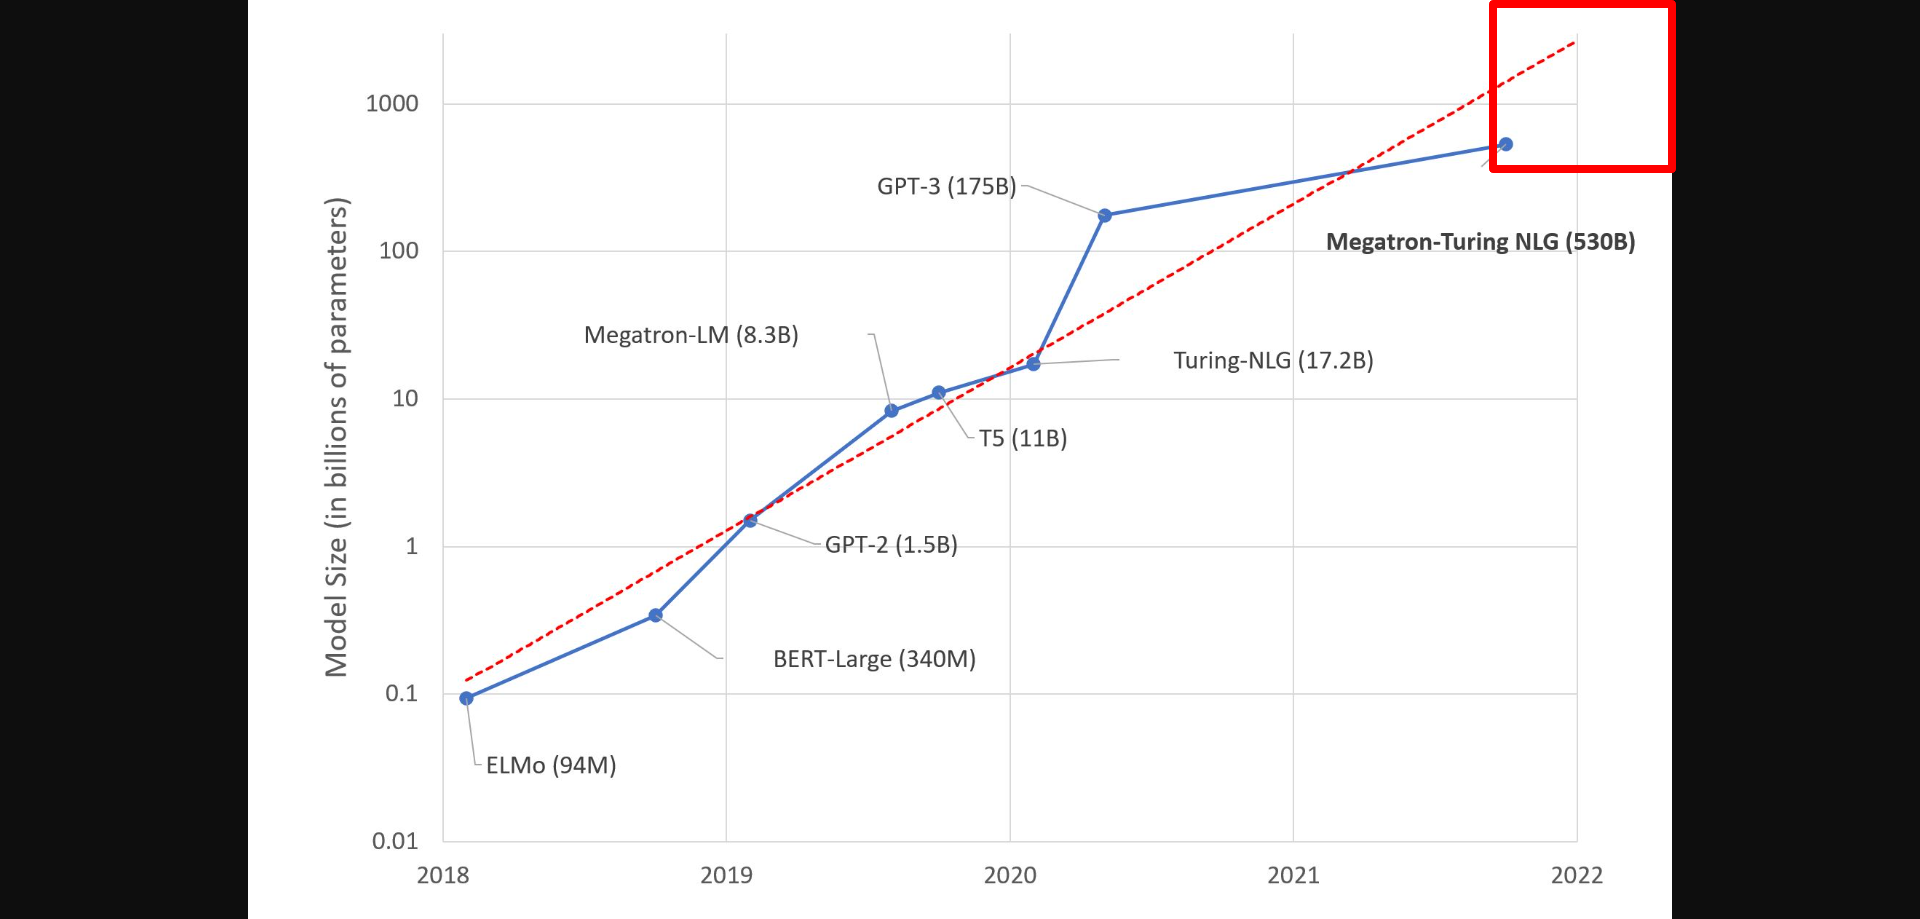
\includegraphics[trim={10cm 0 10cm 0}, clip, height=\textheight]{Figs/ModelSize2.png}
\end{frame}


\begin{frame}
    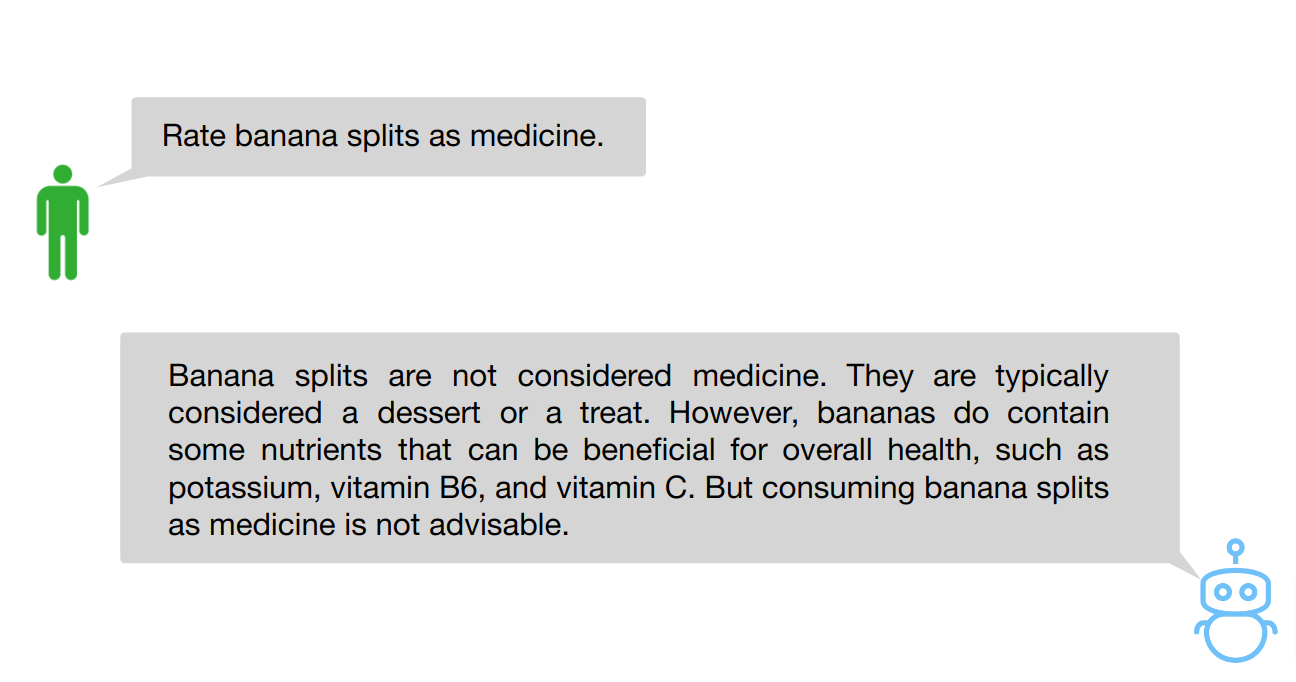
\includegraphics[width=\textwidth]{Figs/Banana.png}
\end{frame}

% \begin{frame}
%     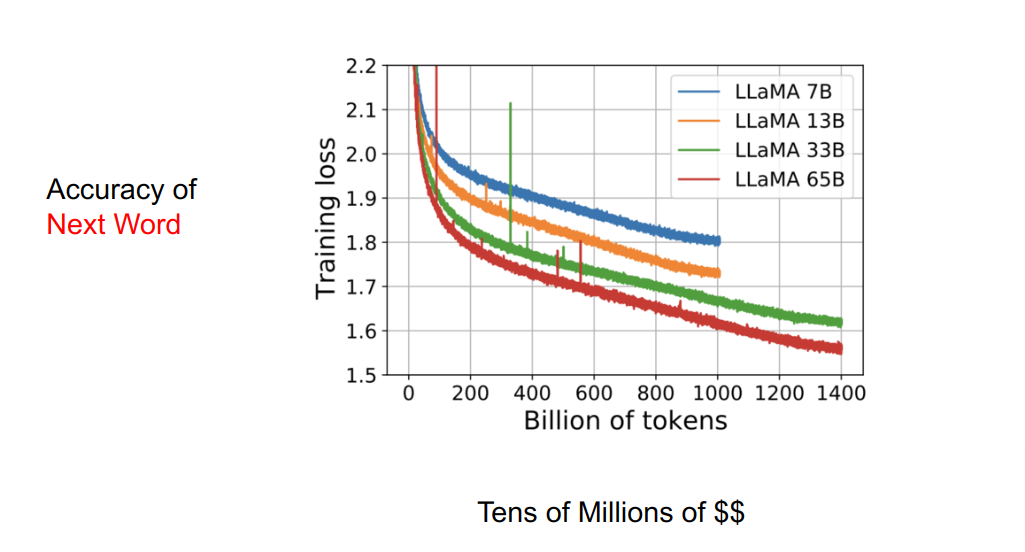
\includegraphics[width=\textwidth]{Figs/llama.png}
% \end{frame}





\begin{frame}{Caveats}
    \begin{itemize}
        \item LLMs are remarkable, we should use them for most things
        \item This talk is \structure{not} about LLMs 
    \end{itemize}
\end{frame}




\begin{frame}
    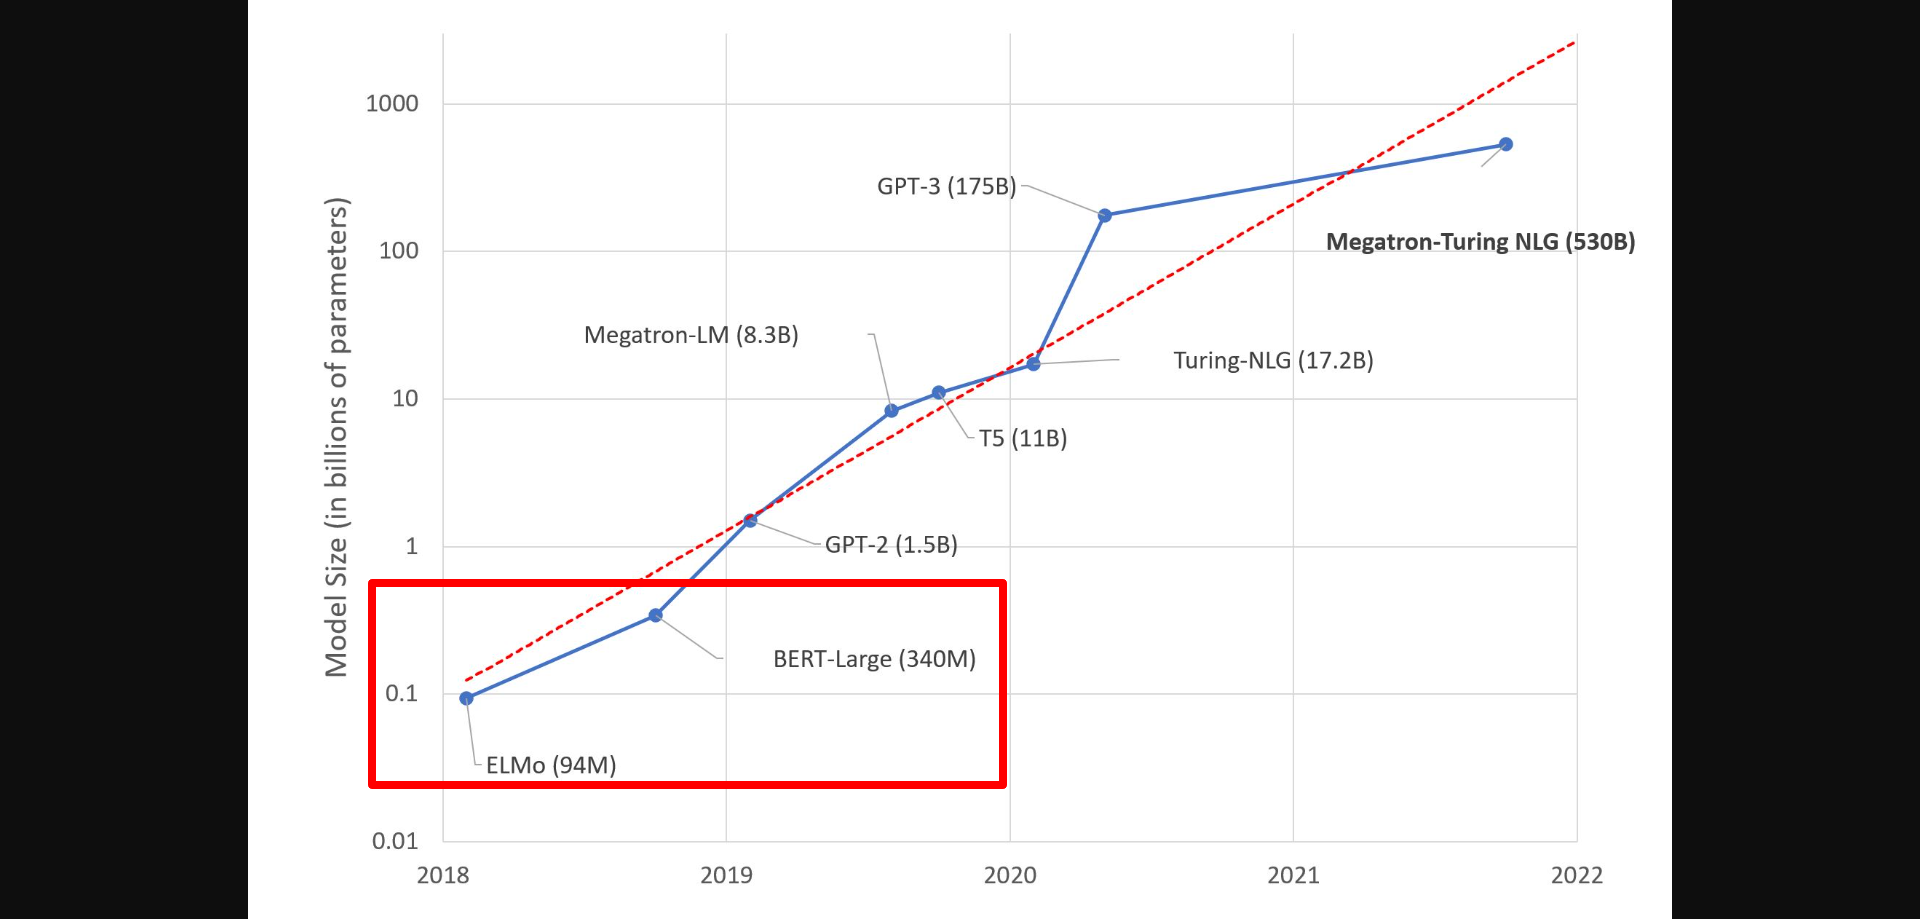
\includegraphics[trim={10cm 0 10cm 0}, clip, height=\textheight]{Figs/ModelSize3.png}
\end{frame}

\begin{frame}{Context}
    \begin{itemize}
        \item BERT used to require non-trivial compute 
        \item Belief: Open architecture questions in NLP
        \item Today's Talk: How important is \textit{attention}?
    \end{itemize}
\end{frame}


\begin{frame}{\textcolor{red}{ELMo} }

    \begin{columns}
    \begin{column}{0.3\linewidth}
    \centerline{Bidirectional RNN}
    \end{column}
    \begin{column}{0.7\linewidth}
    
    \begin{figure}
    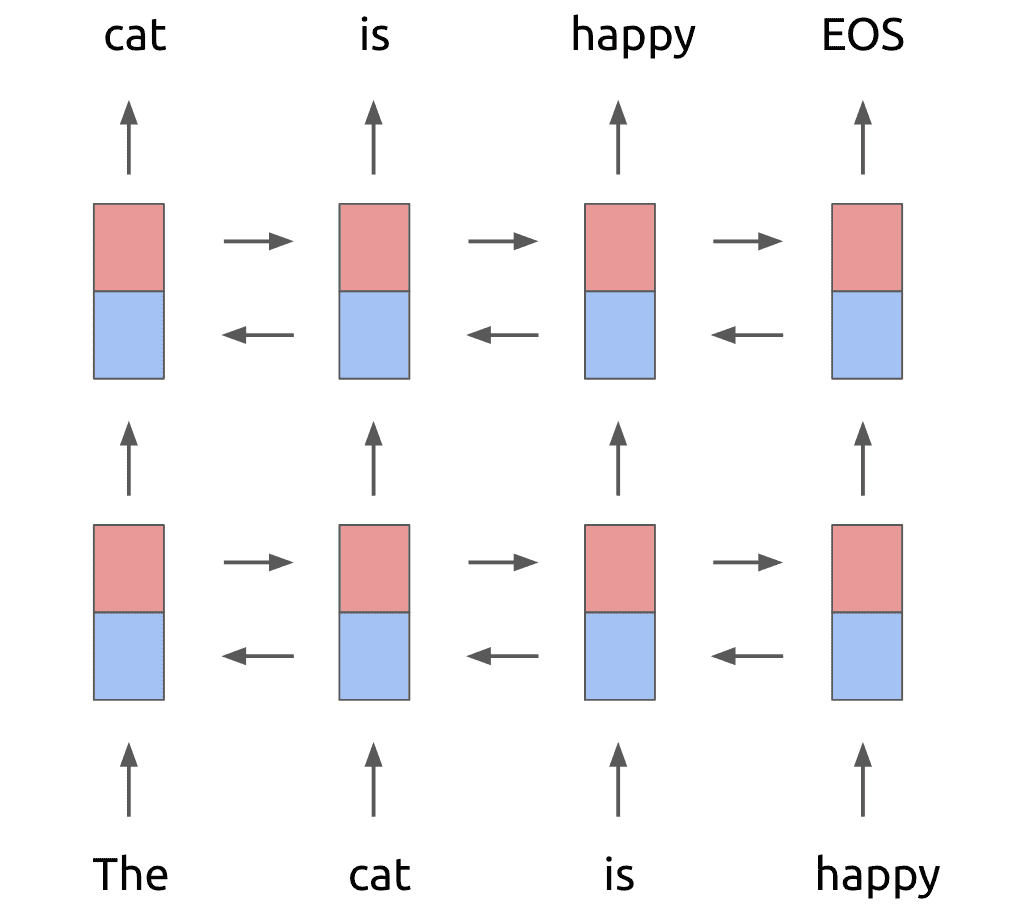
\includegraphics[width=0.8\textwidth]{Figs/elmo.png}
    \end{figure}
    \end{column}
    \end{columns}
    \blfootnote{\cite{DBLP:conf/naacl/PetersNIGCLZ18}}

\end{frame}

\begin{frame}{\textcolor{red}{ELMo} For Pretraining}
    \begin{table}
    \begin{tabular}{lc}
        \toprule
        Model & GLUE\\
        \midrule 
         ELMo& 67.7  \\
         ELMo+Attn&  71.0\\ 
         \visible<2>{BERT-Base & 79 - 83} \\
        \bottomrule
    \end{tabular}
    \end{table}
\blfootnote{\cite{DBLP:conf/naacl/PetersNIGCLZ18, devlin2018bert}}
\end{frame}

\begin{frame}{Architecture?}
    \begin{itemize}
        \item 
    Several confounding differences, e.g. frozen model.
       \item Followup: \textit{To Tune or Not to Tune? Adapting Pretrained Representations to Diverse Tasks} \cite{peters2019tune}
    \pause

     \item  Conclusion: Transformers significantly beat BiLSTMs
    \end{itemize}
\end{frame}

\begin{frame}{Other Models}

    Maybe there are other models

    \vspace{0.5cm}

    \begin{itemize}
        \item Convolutions?
        \item Mixers?
    \end{itemize}
    
%     \textit{Are Pre-trained Convolutions Better than Pre-trained Transformers?}
% \\
% \\
%     Answer: No. 

\end{frame}

\begin{frame}{Pretraining with CNNs}
    \textit{Are Pre-trained Convolutions Better than Pre-trained Transformers?} \cite{tay2020efficient}

    \vspace{0.5cm}
    
    \visible<2>{\structure{Answer: No.}

    \begin{table}
    \begin{tabular}{lc}
        \toprule
        Model & SST-2\\
        \midrule 
         ELMo &  91.8 \\ 
         Best CNN & 92.2  \\
         BERT-Base & 93.5 \\ 
        \bottomrule
    \end{tabular}
    \end{table}
    
    }
  
\end{frame}


% \begin{frame}{Results: CNNs}
%     \begin{table}
%     \begin{tabular}{lc}
%         \toprule
%         Model & SST-2\\
%         \midrule 
%          Best CNN & 92.2  \\
%          ELMo &  91.8 \\ 
%          BERT-Base & 93.5 \\ 
%         \bottomrule
%     \end{tabular}
%     \end{table}
% \end{frame}

\begin{frame}{Pretraining with FNet}
    \textit{FNet: Mixing Tokens with Fourier Transforms} \cite{lee2021fnet}

    \vspace{0.5cm}
    
    Replaces attention with 2D FFT mixing-layer.

    \visible<2>{
    \begin{table}
    \begin{tabular}{lc}
        \toprule
        Model & GLUE (dev)\\
        \midrule 
         Best FNet & 76.3  \\
         BERT-Base & 83.3 \\ 
        \bottomrule
    \end{tabular}
    \end{table}
    }
\end{frame}



\begin{frame}{Transformers are Great...}    
    \begin{itemize}
        \item Highly optimized training 
        \item Long-range ability
        \item Expensive $O(n^2)$, but we have the money...
    \end{itemize}
    \vspace{0.5cm}

    \visible<2>{(But aren't you curious...)}
\end{frame}

\section{State Space Models}
\begin{frame}{Outline}
    \tableofcontents[currentsection]
\end{frame}


\begin{frame}{State Space Models (SSM)}
    \begin{itemize}
        
        \item Think hybrid RNN / CNN 
        
        \item SOTA on speech generation and long-range tasks 

        \item Tutorial at \textit{The Annotated S4}
    \end{itemize}

    \blfootnote{\cite{gu2020hippo,gu2021combining,gu2021efficiently}}
\end{frame}


\begin{frame}{State Space Model - Continuous Time}
    Let $u(t) \in \mathbb{R}$ be a continuous input and $y(t) \in \mathbb{R}$ be output. 

\pause
\vspace{0.5cm}

SSM is a differential equation.
\begin{align*}
    \boldsymbol{x}'(t) &= \boldsymbol{A}\boldsymbol{x}(t) + \boldsymbol{B}u(t) \\  
    y(t) &= \boldsymbol{C}\boldsymbol{x}(t) + \boldsymbol{D}u(t).
\end{align*}

\pause 
Where $\boldsymbol{x}(t) \in \mathbf{R}^N$ is a hidden state and model \structure{parameters},

$$\boldsymbol{A} \in \mathbb{R}^{N\times N}, \boldsymbol{B}\in \mathbb{R}^{N \times 1}, \boldsymbol{C} \in \mathbb{R}^{1 \times N}, \boldsymbol{D} \in \mathbb{R}^{1\times 1}$$

\end{frame}
\begin{frame}{Discrete Time Sequence}

Goal: Map scalar sequence $u_{1}, \ldots, u_L$ to $y_1, \ldots, y_L$,

\begin{figure}
    \centering
    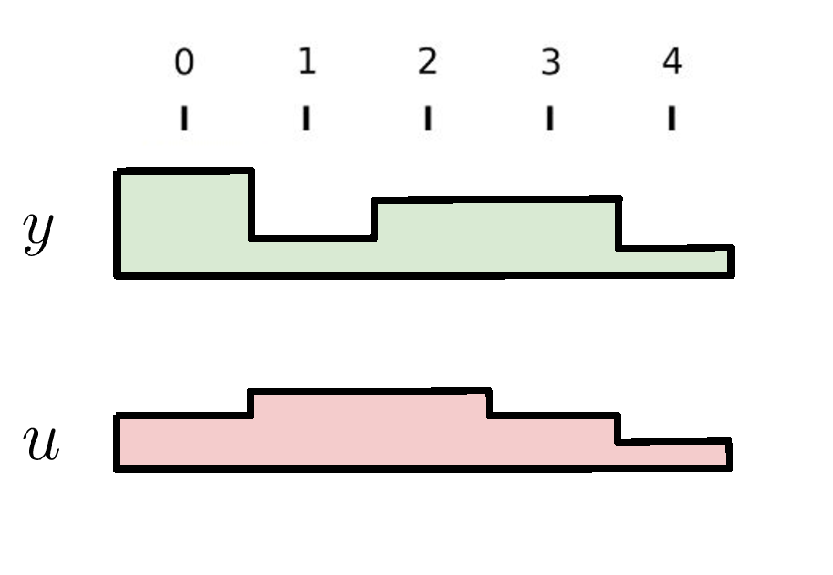
\includegraphics[width=0.5\textwidth]{Figs/SSMStart.pdf}
    \label{fig:my_label}
\end{figure}
\end{frame}

\begin{frame}{Discrete Time SSM}

SSM on discretize time data,

\begin{align*}
\boldsymbol{x}_{k} &= \boldsymbol{\overline{A}} \boldsymbol{x}_{k-1} + \boldsymbol{\overline{B}} u_k \\ 
y_k &= \boldsymbol{\overline{C}} \boldsymbol{x}_{k \phantom{- 1}} + \boldsymbol{\overline{D}}  u_k. 
\end{align*}

Using discretization with (learned) sampling rate parameter $\Delta$, 

$$\boldsymbol{\overline{A}}, \boldsymbol{\overline{B}}, \boldsymbol{\overline{C}}  = \text{discretize}(\boldsymbol{A}, \boldsymbol{B}, \boldsymbol{C}, \Delta )$$

\end{frame}

\begin{frame}{Recurrent Form}

Output sequence $y_1, \ldots, y_L$ can be computed as a linear RNN,

\begin{align*}
\boldsymbol{x}_{k} &= \boldsymbol{\overline{A}} \boldsymbol{x}_{k-1} + \boldsymbol{\overline{B}} u_k \\ 
y_k &= \boldsymbol{\overline{C}} \boldsymbol{x}_{k \phantom{- 1}} + \boldsymbol{\overline{D}}  u_k. 
\end{align*}

Note $\boldsymbol{x}_k \in \mathbb{R}^N$ is the bigger hidden state for $u_k \in \mathbb{R}$, and $\boldsymbol{x}_0 = \mathbf{0}$.

\end{frame}

\begin{frame}{Convolutional Form}

Alternative: 1D convolution with kernel $\boldsymbol{\overline{K}}$ (width $L$),

\begin{align*}
\overline{K} &= (\boldsymbol{\overline{C}}\boldsymbol{\overline{B}}, \boldsymbol{\overline{C}}\boldsymbol{\overline{A}}\boldsymbol{\overline{B}}, \dots, \boldsymbol{\overline{C}}\boldsymbol{\overline{A}}^{L-1}\boldsymbol{\overline{B}}) \\
y &= \text{conv1d}(\overline{K}_L \ldots \overline{K}_1, u_1 \ldots u_L)
\end{align*}

Intuition: 
\pause
$$y_1 = \boldsymbol{\overline{C}} \boldsymbol{\overline{B}} u_1$$ 
\pause
$$y_2 = \boldsymbol{\overline{C}} \boldsymbol{\overline{A}} \boldsymbol{\overline{B}} u_1 + \boldsymbol{\overline{C}} \boldsymbol{\overline{B}} u_2 = \boldsymbol{\overline{C}} (\boldsymbol{\overline{A}} \boldsymbol{\overline{B}} u_1 + \boldsymbol{\overline{B}} u_2) = \boldsymbol{\overline{C}} (\boldsymbol{x}_1 + \boldsymbol{\overline{B}} u_2) $$
\end{frame}

\begin{frame}{Convolutional Form}
Step 1: Discretize (Training Only). Step 2: Apply 1D Conv
\begin{figure}
    \centering
    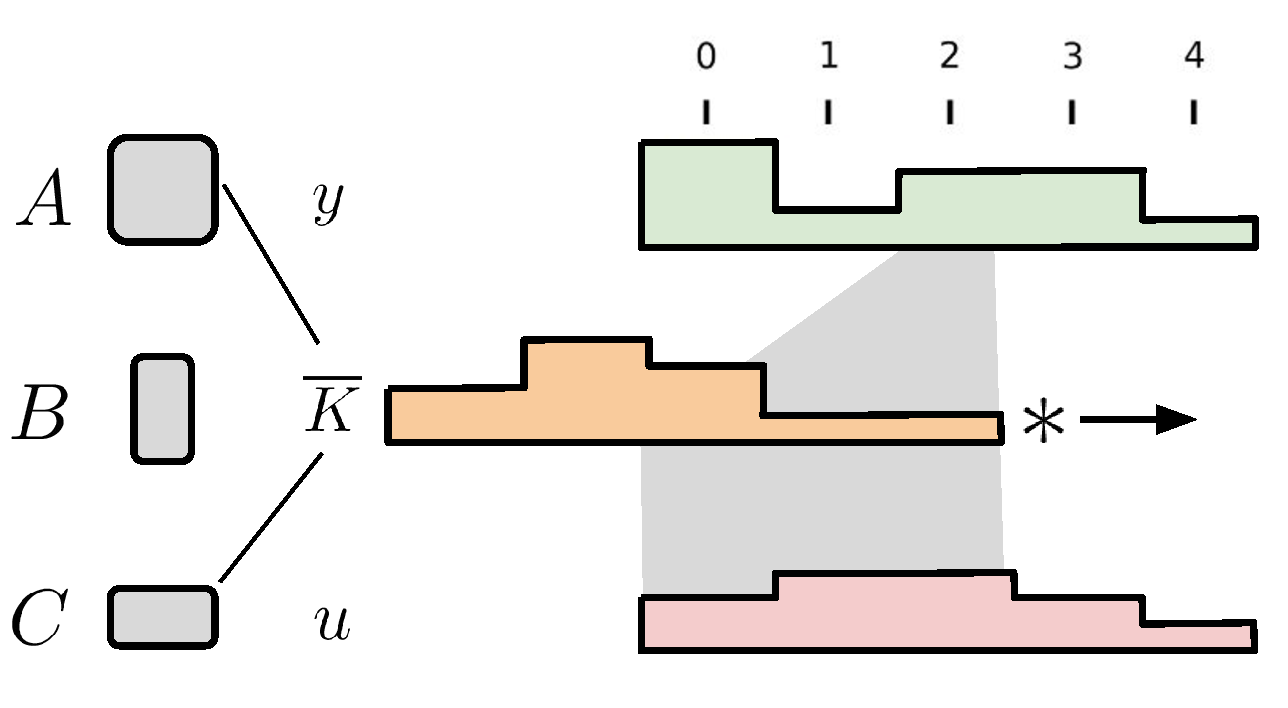
\includegraphics[width=0.6\textwidth]{Figs/SSMSide.pdf}
    \label{fig:my_label}
\end{figure}
\end{frame}

\begin{frame}{Implementation - Computing Kernel}
    
    $$\boldsymbol{\overline{K}} = (\boldsymbol{\overline{C}}\boldsymbol{\overline{B}}, \boldsymbol{\overline{C}}\boldsymbol{\overline{A}}\boldsymbol{\overline{B}}, \dots, \boldsymbol{\overline{C}}\boldsymbol{\overline{A}}^{L-1}\boldsymbol{\overline{B}}) $$
    
\begin{itemize}    
    \item Simple approximations work well (See S4D, DSS)   
\end{itemize}
\blfootnote{\cite{gu2021efficiently,gupta2022diagonal,gu2022parameterization}}
\end{frame}


\begin{frame}{Implementation - Fourier Transform}
\begin{align*}
&y = \boldsymbol{\overline{K}} \ast u
\end{align*}
\begin{itemize}
    \item At long $L$, convolution computed with FFT.
    \item More efficient than self-attention or standard RNN. 
\end{itemize}
\end{frame}


\begin{frame}{Important Training Initialization}
\begin{itemize}
\item Parameter $\boldsymbol{A}$ is initialized with  HiPPO Matrix \cite{gu2020hippo}

% \begin{scriptsize}
% \begin{align*}  
% \boldsymbol{A}_{nk}= -
% \begin{cases} 
% (2n+1)^{1/2}(2k+1)^{1/2} & \text{if } n > k \\ n+1 &\text{if } n=k \text{\ else\ } 0
% \end{cases} 
% \end{align*}
% \end{scriptsize}


    \item Kernel formed by Legendre coefficients 
\end{itemize}
\begin{figure}
    \centering
    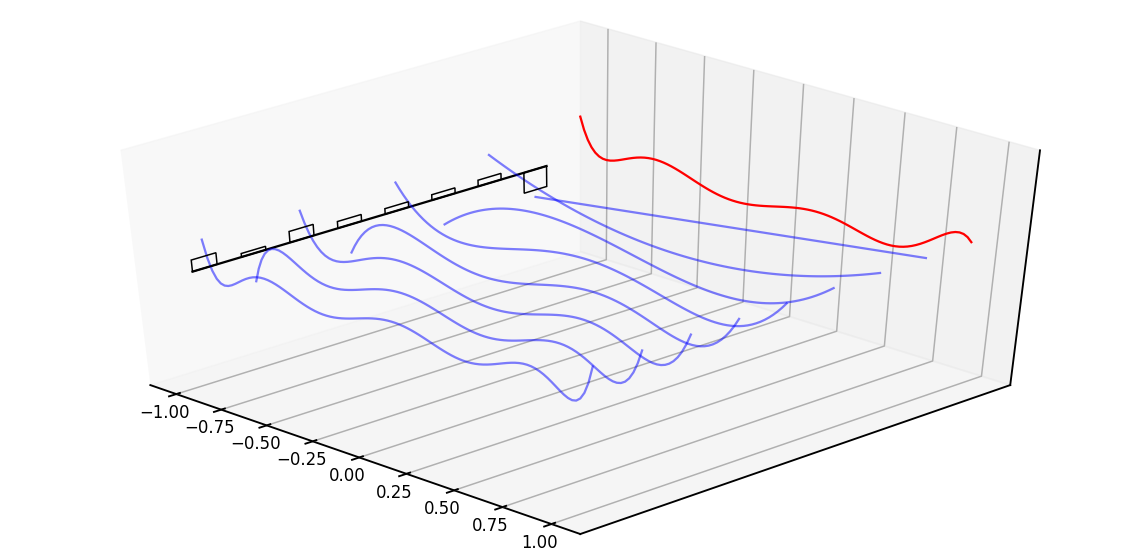
\includegraphics[width=0.7\textwidth]{Figs/hippo.png}
\end{figure}
\end{frame}



\begin{frame}{Summary: SSM}
    \begin{itemize}
        \item Mapping from sequence-to-sequence
        \item Acts like an RNN, Computed like a CNN
        \item Fast to train and utilize
    \end{itemize}
\end{frame}

\section{Model Architectures}
\begin{frame}{Outline}
    \tableofcontents[currentsection]
\end{frame}

\begin{frame}{Objective: Replicate BERT with SSM}
\begin{itemize}
    \item Everything else identical (loss, number of parameters, data) 
\end{itemize}
\end{frame}

% \begin{frame}{Architectures for Pretraining}
%     \begin{itemize}
%         \item Idea 1: Just replace self-attention
%         \item Minimal change to Transformer arch 
%     \end{itemize}
% \end{frame}


\begin{frame}{\structure{Naive Idea}: Self-attention $\Rightarrow$ SSM}
\begin{figure}
    \centering
    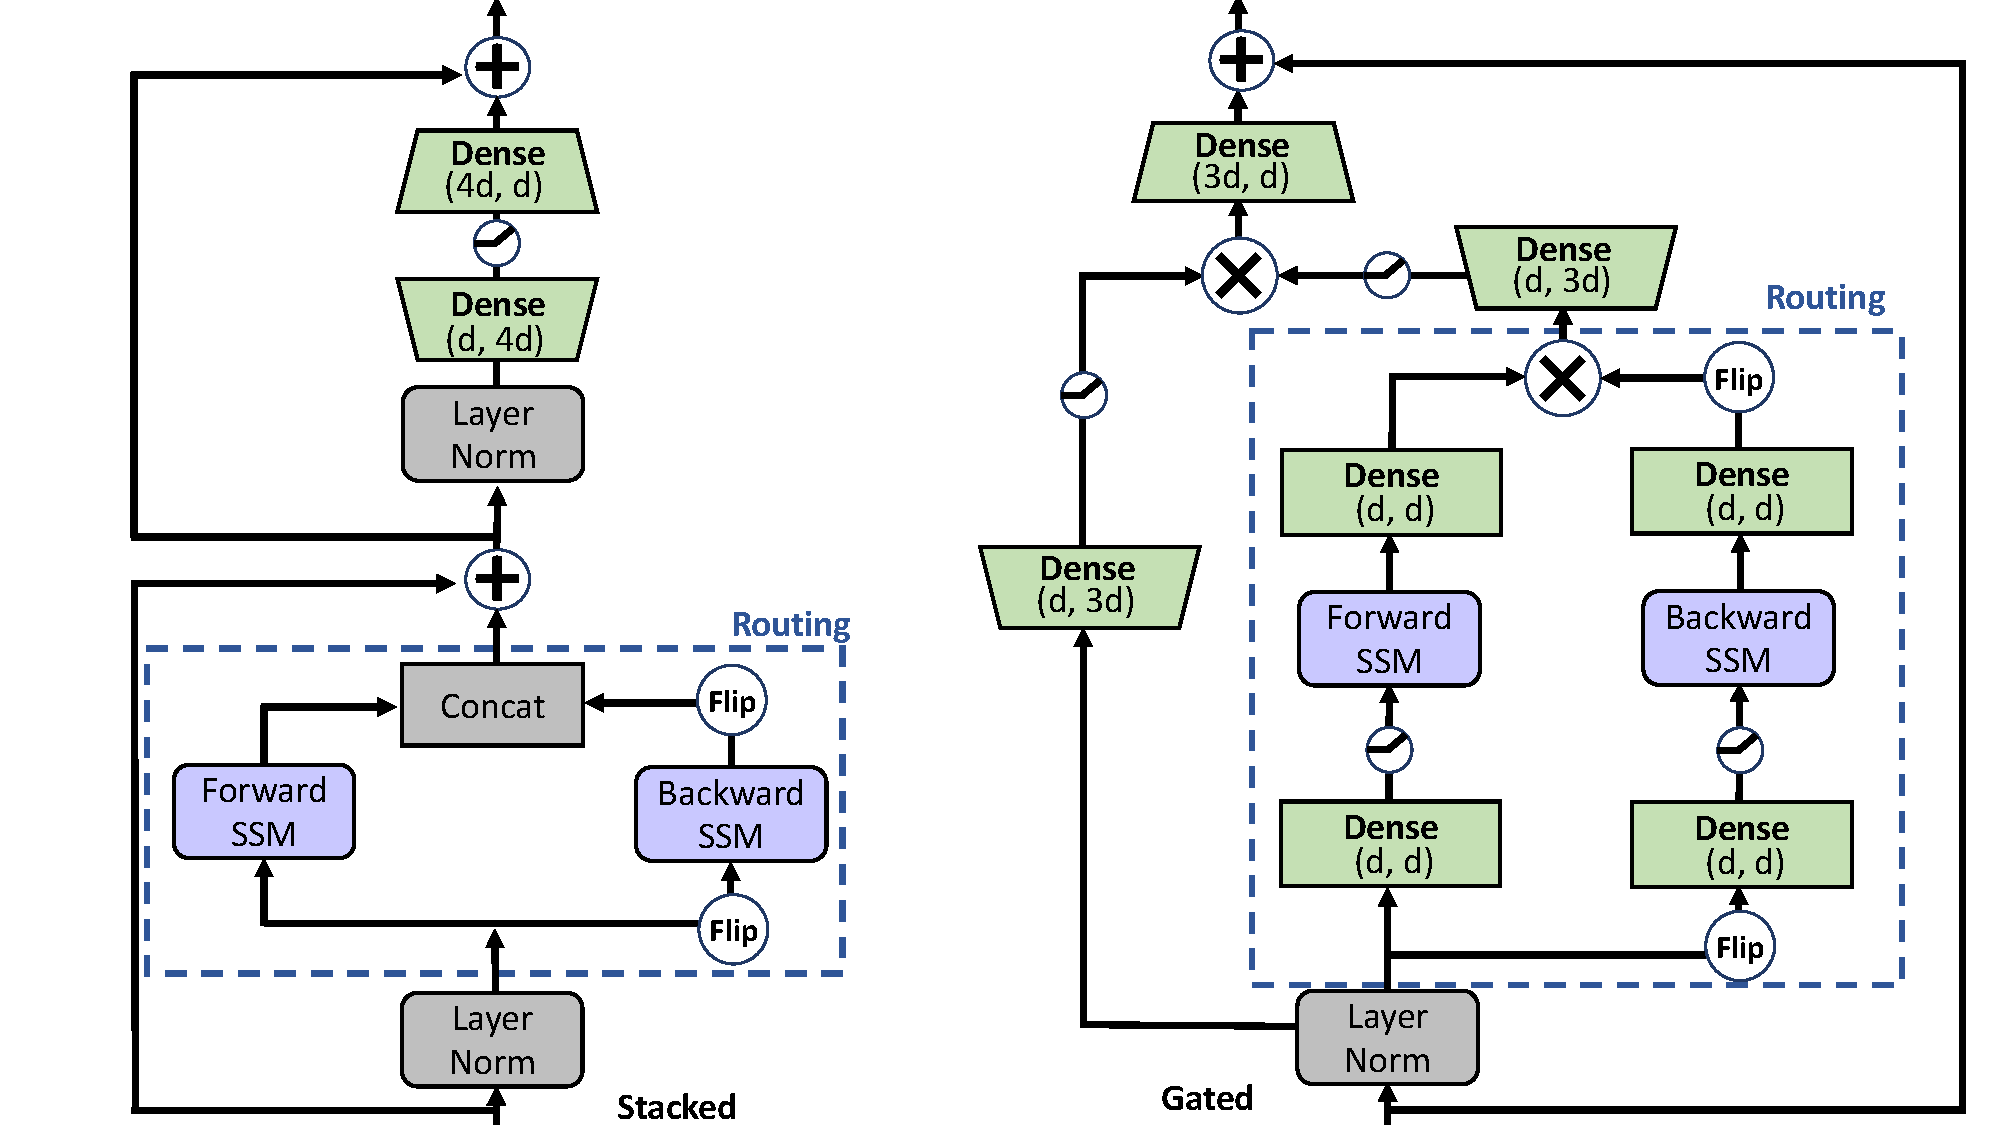
\includegraphics[height=0.8\textheight,trim={0 0 18cm 0},clip]{Figs/model_architecture_comparison2.pdf}
    \caption{}
    \label{}
\end{figure}
\end{frame}

\begin{frame}{Can this work?}
\begin{itemize}
    \item SSM is significantly less expressive than self-attention.     
    \item Static routing through the model like a CNN.
    \item Can it learn to do \structure{matching} across sentences?
\end{itemize}
\pause 
\vspace{0.5cm}




\end{frame}


\begin{frame}{Test: Matching Across Gaps}
\centerline{Task: QNLI \cite{wang2018glue}}
\vspace{0.5cm}

   
    \centerline{\textcolor{red}{What percentage of farmland grows wheat?}}
    
    \centerline{$\sim \sim \sim $}

    \centerline{\textcolor{olivegreen}{More than 50\% of this area is sown for wheat and 33\% for barley.}}
    
    \pause
    
    \begin{table}[t]
\center
    \begin{tabular}{ccc}
    \toprule
    \centering
     Arch  & \textcolor{red}{H} P &   \textcolor{red}{H} $\sim$ P \\    
    \midrule
             \textsc{stack} / \textsc{ssm} & 77.4 &  69.7\\
          % \textsc{gated} / \textsc{ssm} & 77.4 &  77.7\\
    \bottomrule
    \end{tabular}
    \caption{}
    \label{tab:synthetic}
\end{table}
\end{frame}



% \begin{frame}{Does this work}
    
% \end{frame}



\begin{frame}{\structure{Proposed Fix}: Multiplicative Gating}

Add dynamism to stacked model with multiplicative gating.

$$\sigma(\mathbf{W} \mathbf{u}) \otimes (\mathbf{V} \mathbf{u})$$

Positive results with CNN, Transformer, and SSM models.


\blfootnote{\cite{dauphin2017language, shazeer2020glu, narang2021transformer}}

\end{frame}

\begin{frame}{Proposed Architecture: BiGS}
\begin{figure}
    \centering
    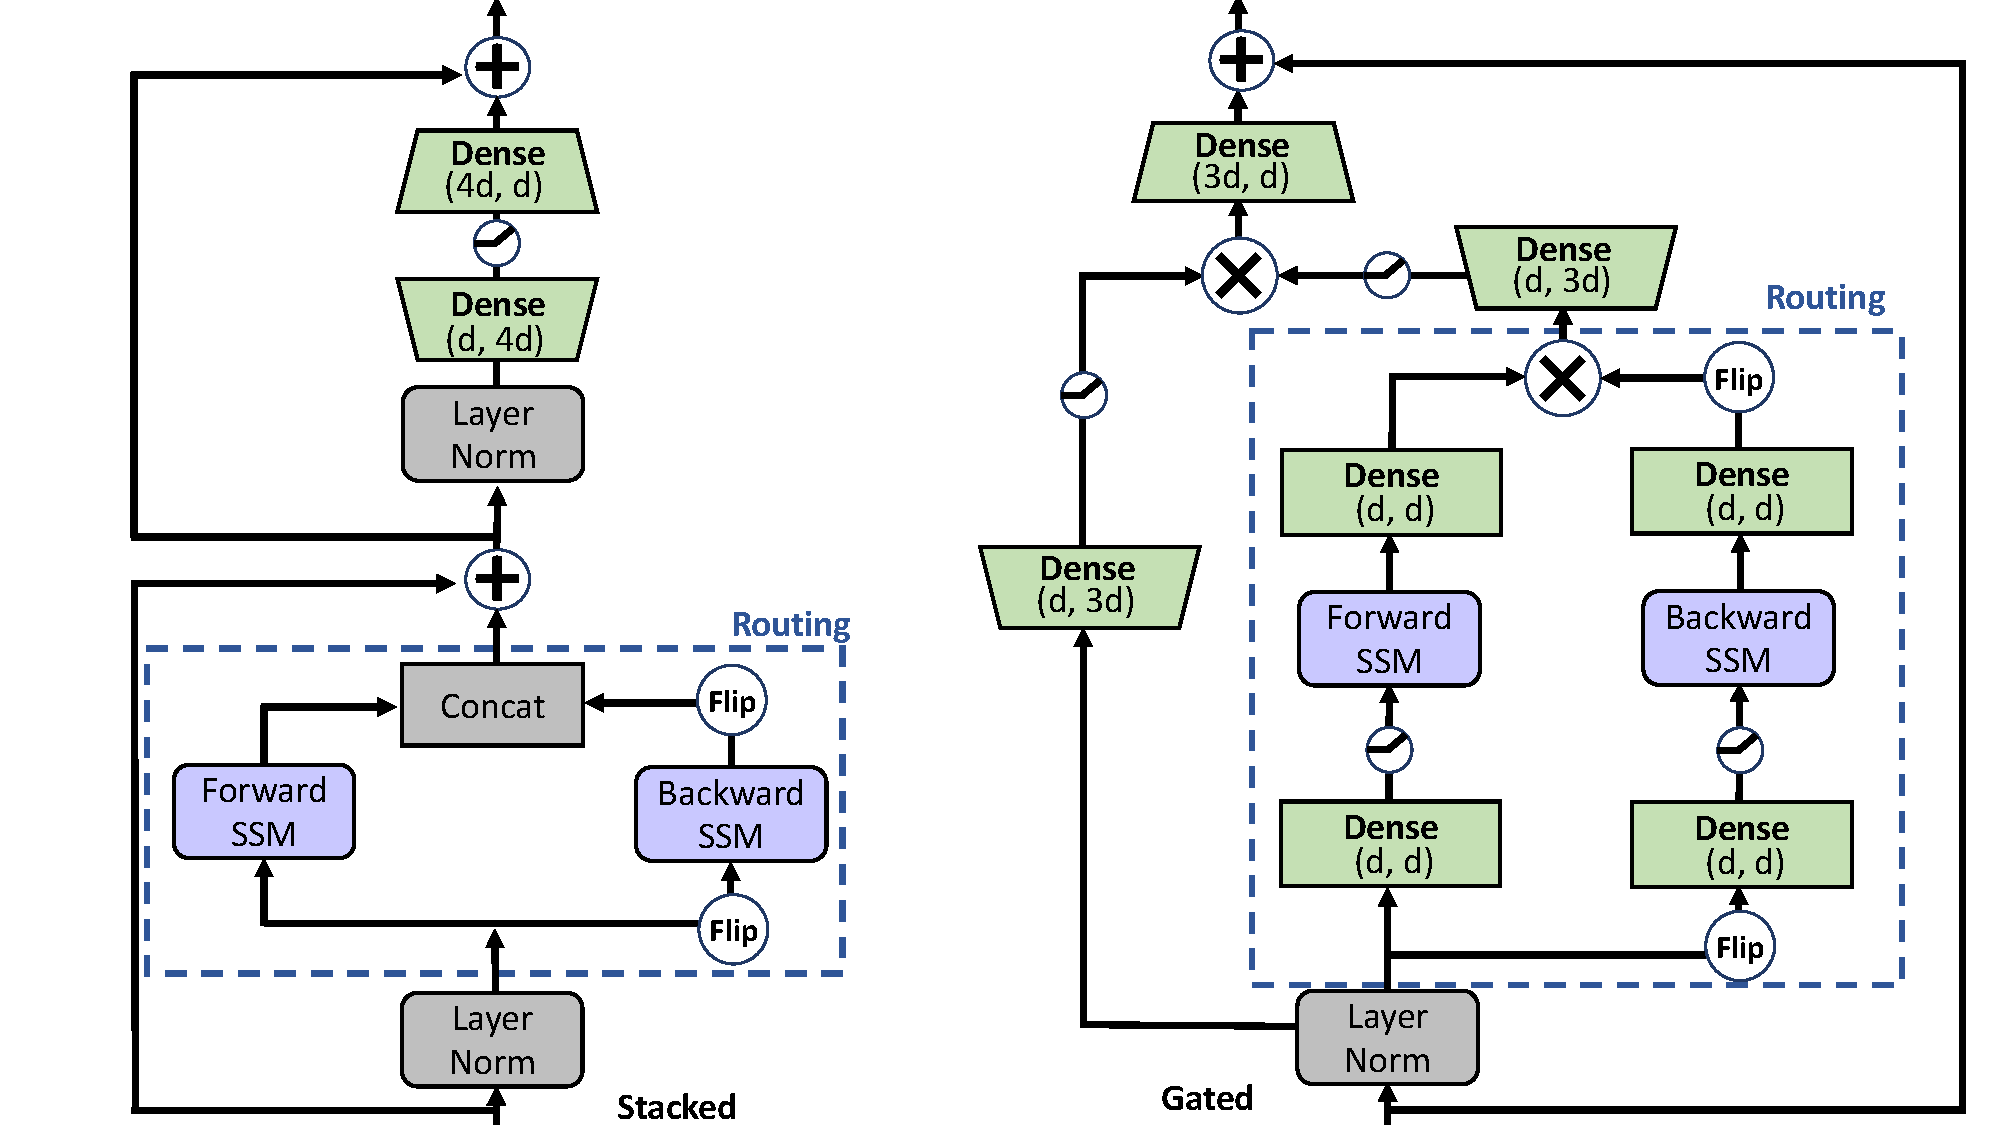
\includegraphics[height=0.7\textheight,trim={16cm 0 0 0},clip]{Figs/model_architecture_comparison2.pdf}
    \caption{}
    \label{fig:my_label}
\end{figure}
\end{frame}

\begin{frame}{Gating Adaptation}
   \centerline{\textcolor{red}{What percentage of farmland grows wheat?}}
    
    \centerline{$\sim \sim \sim $}

    \centerline{\textcolor{olivegreen}{More than 50\% of this area is sown for wheat and 33\% for barley.}}


    \begin{table}[t]
\center
    \begin{tabular}{lcc}
    \toprule
    \centering
     Arch  & \textcolor{red}{H} P &   \textcolor{red}{H} $\sim$ P \\      
    \midrule
               \textsc{stack} / \textsc{ssm} & 77.4 &  69.7\\
         \textsc{gated} / \textsc{ssm} & 77.4 &  77.7\\
    \bottomrule
    \end{tabular}
    \caption{ }
    \label{tab:synthetic}
\end{table}
\pause 


\end{frame}

\begin{frame}{Full Experiment: QNLI}

Preview: Experimental results, pretraining for QNLI.

\begin{figure}
    \centering
    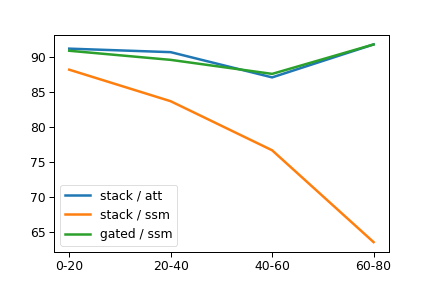
\includegraphics[height=0.7\textheight]{Figs/graph.png}
    \label{fig:my_label}
\end{figure}
\end{frame}

\begin{frame}{Related Result: Induction Heads (H3)}
    Synthetic \structure{induction head} experiment from \cite{dao2022hungry}

    \vspace{0.5cm}
    
    \centerline{a b c d e $\Rightarrow$ f g h i . . . x y z $\Rightarrow$  \ \ \ \  \textcolor{red}{f} }

    \begin{table}[t]
\center
    \begin{tabular}{lcc}
    \toprule
    \centering
     Arch  & Induction \\    
    \midrule
                \textsc{ssm} & 35.6 \\
         \textsc{gating} + \textsc{ssm} & 100\\
         \textsc{attention} & 100\\
    \bottomrule
    \end{tabular}
    \caption{ }
    \label{tab:synthetic}
\end{table}
\end{frame}


\begin{frame}{Induction Heads}

\begin{columns}
    \begin{column}{0.5\textwidth}
    \begin{figure}
        \centering
        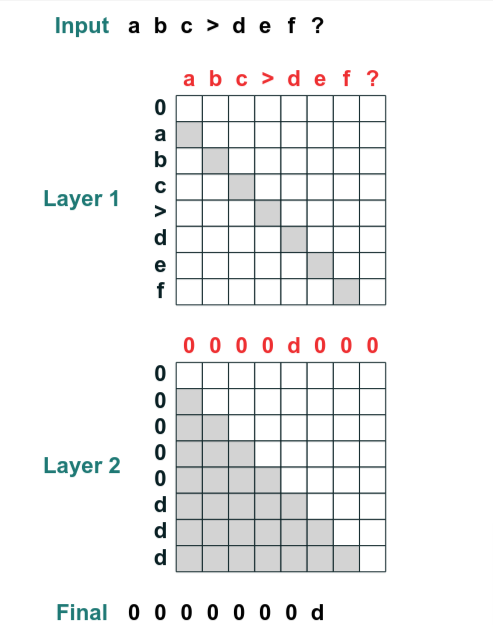
\includegraphics[height=0.8\textheight]{Figs/induct.png}
        
        \label{fig:my_label}
    \end{figure}        
    \end{column}    
    \begin{column}{0.5\textwidth}
    \begin{figure}
        \centering

        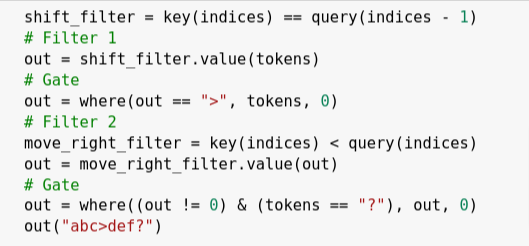
\includegraphics[height=0.3\textheight]{Figs/RASP.png}
        \label{fig:my_label}
    \end{figure}        
    \end{column}    
\end{columns}

\end{frame}



% \begin{frame}{Gating}

% \end{frame}

% \begin{frame}{Simpler multiplicative Interactions}
% \begin{figure}
%     \centering
%     % 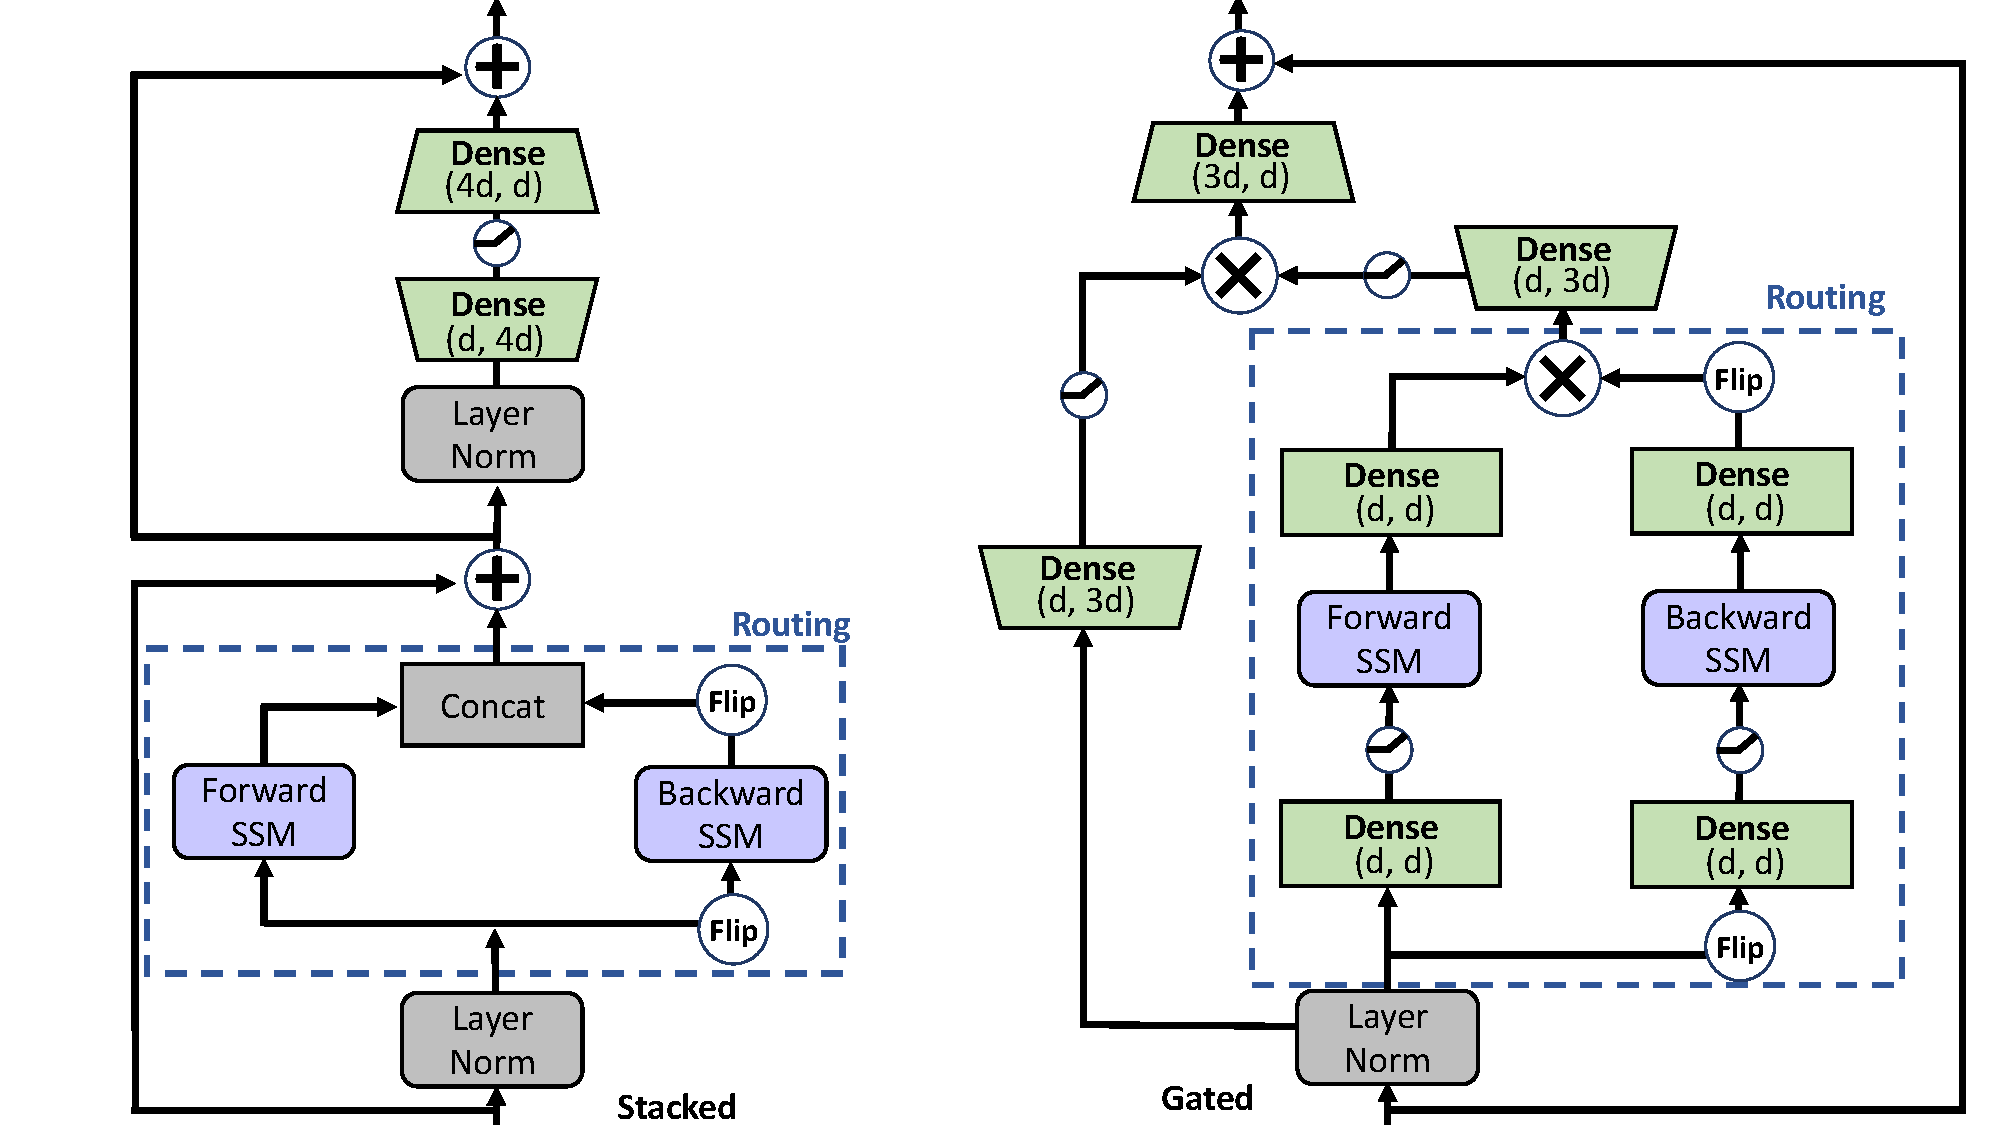
\includegraphics{Figs/model_architecture_comparison2.pdf}
%     \caption{Caption}
%     \label{fig:my_label}
% \end{figure}
% \end{frame}

\section{Experiments}

\begin{frame}{Outline}
    \tableofcontents[currentsection]
\end{frame}


\begin{frame}{\structure{Experiment 1:} BERT}
\begin{itemize}
    \item Models trained using ``24 Hour'' BERT \cite{izsak2021train}
    \begin{itemize}
        \item All BERT-Large Size
        \item Training length (Short 11B, Medium 22B, Full >100B)
        \item 128 Length Sequences
    \end{itemize}
    
    \item Codebase in JAX (from Annotated S4 {\small \cite{rush2022s4}}) using S4D
    \item Training data and masking is identical
\end{itemize}
\end{frame}

% \begin{frame}{Short Training $\sim$11B Tokens}
%     \begin{table}
%     \begin{tabular}{lc}
%         \toprule
%         Model & GLUE (Dev)\\
%         \midrule 
%          BERT &  84.1\\ 
%          Stacked-SSM & 77.2 \\ 
%          BiGS & 84.0 \\
%         \bottomrule
%     \end{tabular}
%     \end{table}
% \end{frame}

\begin{frame}{Short Training $\sim$11B Tokens}
    \begin{table}
    \begin{tabular}{lc}
        \toprule
        Model & GLUE (Dev)\\
        \midrule 
         ELMo & 68.7 \\
         BERT &  84.1\\ 
         Stacked-SSM & 77.2 \\ 
         BiGS & 84.0 \\
        \bottomrule
    \end{tabular}
    \end{table}
\end{frame}

\begin{frame}{Is it just Gating?}
    \begin{table}
    \begin{tabular}{lc}
        \toprule
        Model & GLUE \\
        \midrule 
         BERT &  84.1\\ 
         Gated-BERT &  82.6 \\ 
        \bottomrule
    \end{tabular}
    \end{table}
\end{frame}


\begin{frame}{BERT Large > 100B Tokens}
    \begin{table}
    \begin{tabular}{lc}
        \toprule
        Model & GLUE (Test)\\
        \midrule 
         BERT-Large^* &  83.0\\ 
         BiGS & 83.0 \\
        \bottomrule
    \end{tabular}
    \end{table}
    \centerline{$^*$Best reported BERT-Large Results.}
\end{frame}

\begin{frame}{Analysis: Masked PPL Transfer}
    \begin{figure}
    \centering
    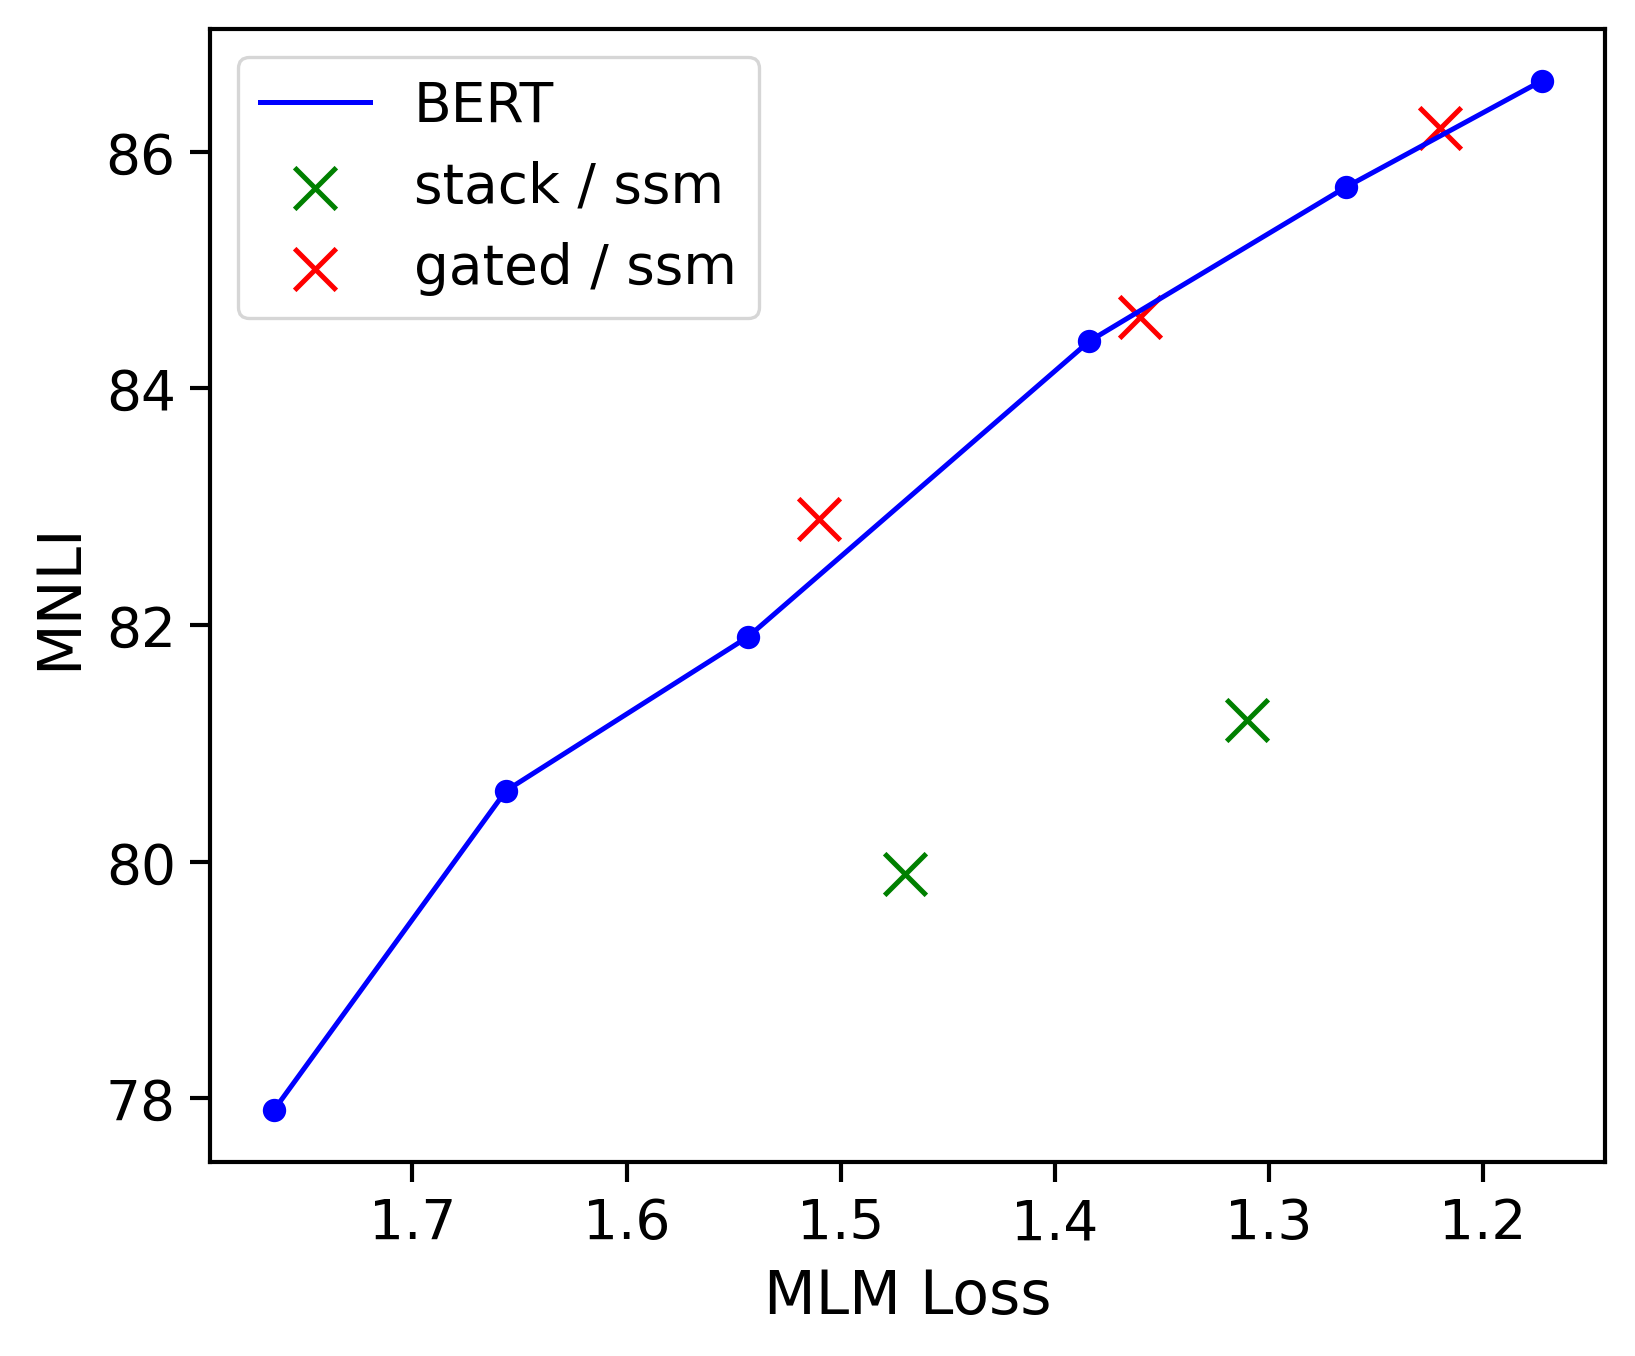
\includegraphics[width=0.6\textwidth]{Figs/MNLI.png}
\end{figure}
\end{frame}

\begin{frame}{Analysis: Kernel Visualization}


\begin{figure}
    \centering
    \includegraphics[width=\textwidth]{Figs/kernel1.png}
\end{figure}

\begin{itemize}
    \item Each BiGS layer only has 2 kernels (forward / backward). 
    \item Shows \structure{all routing} in layer 2! (vs $O(HT^2)$ attention coef.)
\end{itemize}


\end{frame}

\begin{frame}{Analysis: All Kernels}
\begin{figure}
    \centering
    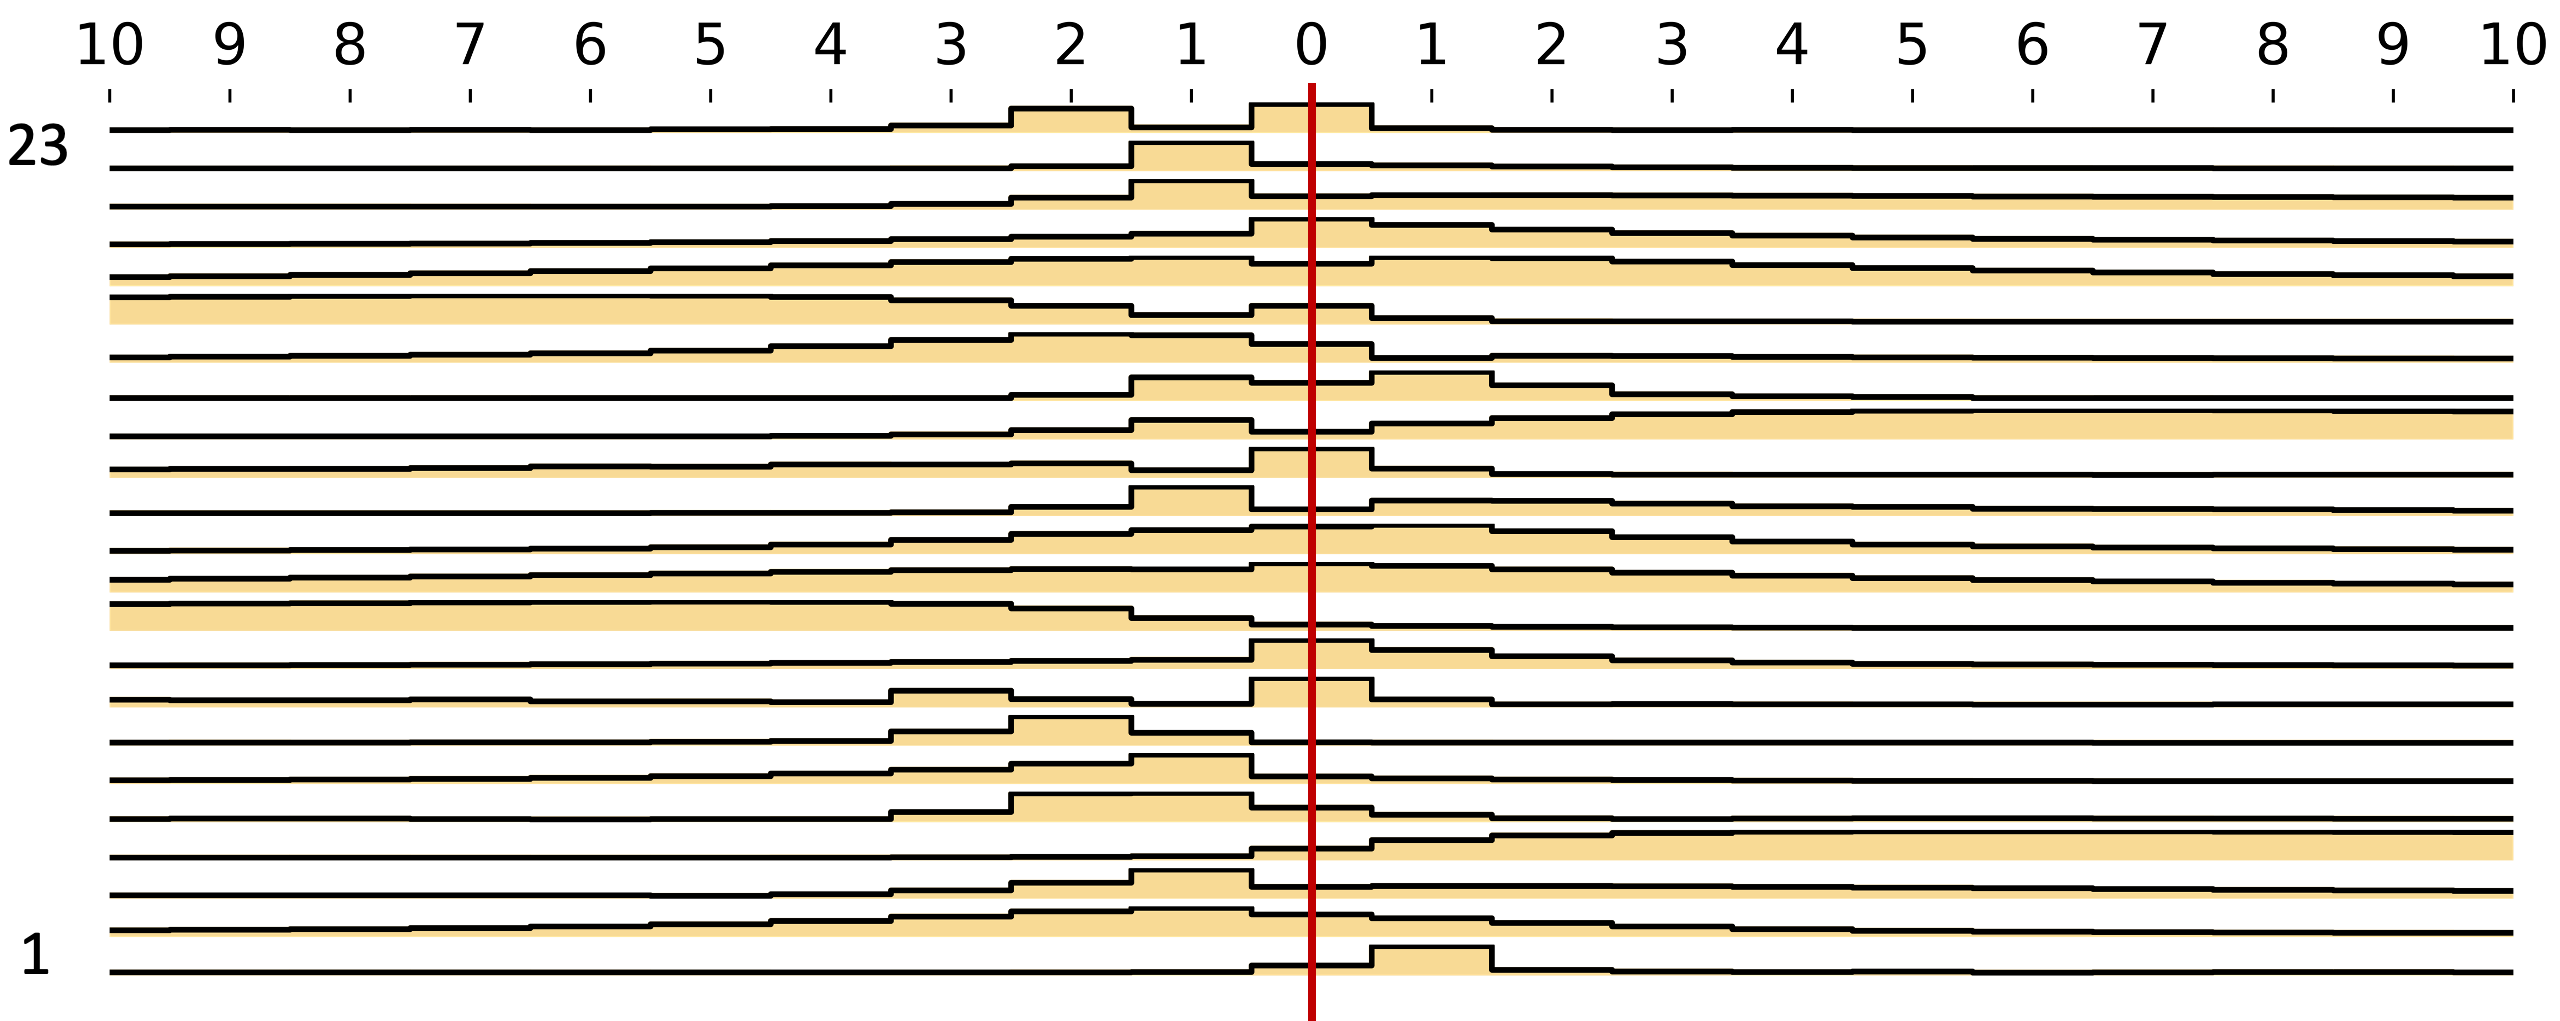
\includegraphics[height=0.6\textheight]{Figs/kernel2.png}
\end{figure}
\end{frame}

\begin{frame}{Analysis: Change in Kernels during Finetuning }

\centerline{Task: MNLI}
\begin{figure}
    \centering
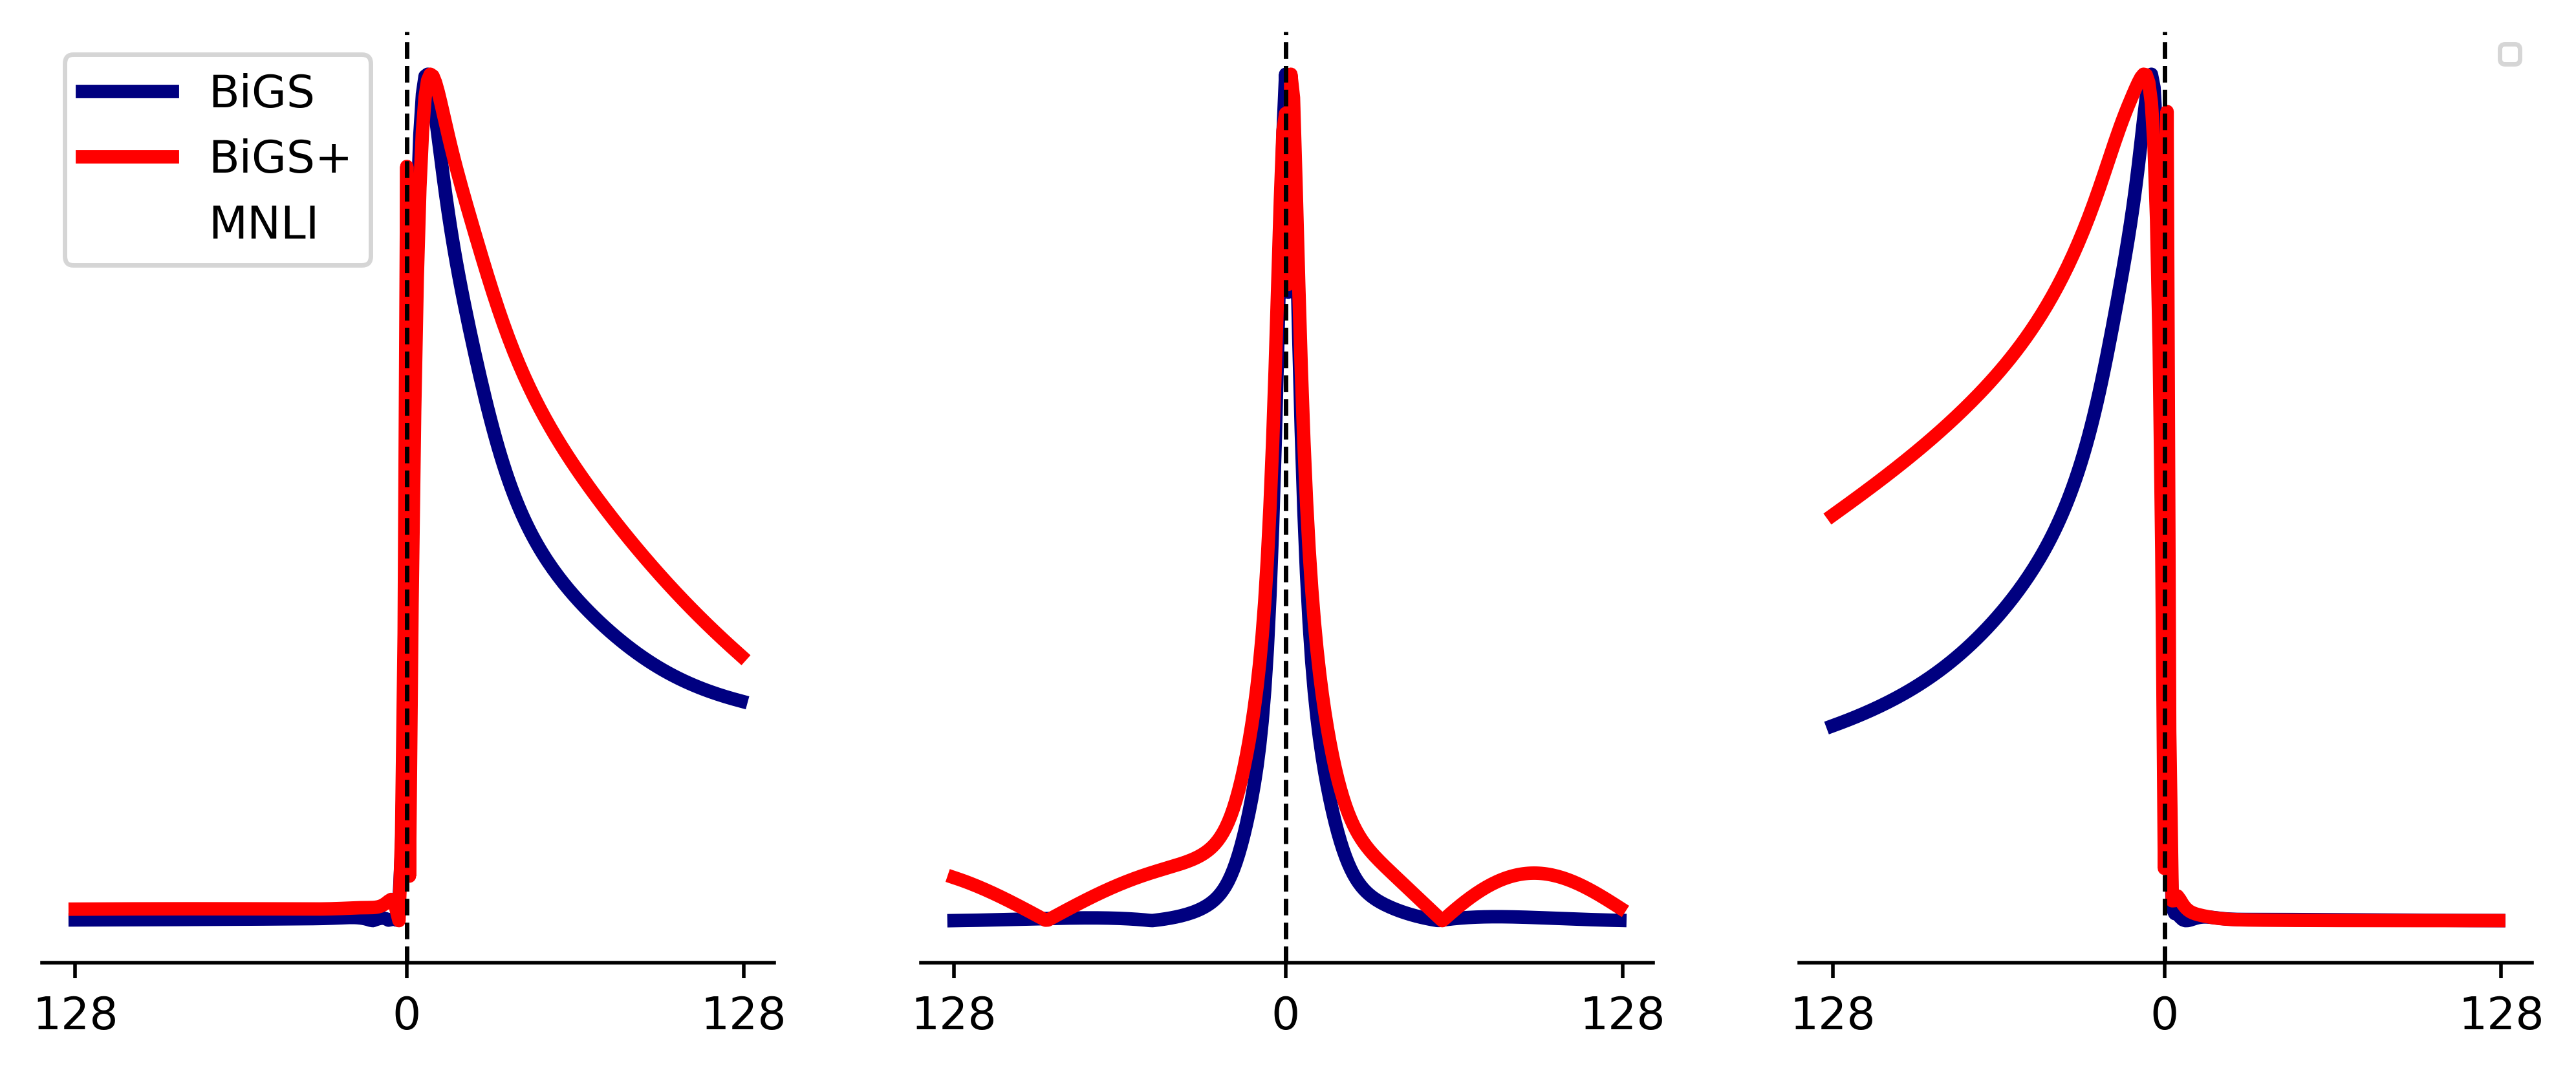
\includegraphics[width=0.8\textwidth]{Figs/comparison_results.png}
    \end{figure}
\end{frame}

\begin{frame}{Analysis: Syntax}
\begin{itemize}
    \item Observation: SSM model seems to do better on syntax-centric tasks 
    \item Hypothesis: Locality of features encourages a stack-like inductive bias. 
\end{itemize}
\end{frame}

\begin{frame}{\structure{Observation 1}: COLA}
    \begin{table}
    \begin{tabular}{lc}
        \toprule
        Model & COLA \\
        \midrule 
         BERT &  60.5\\ 
         BiGS &  64.7 \\ 
        \bottomrule
    \end{tabular}
    \end{table}
    Statistically significant across runs.
\end{frame}


\begin{frame}{\structure{Observation 2}: Agreement Attractors}
    Task from \cite{linzen2016assessing,goldberg2019assessing}.
\vspace{0.5cm}

    \begin{quote}        
    Yet the \textbf{ratio} of \underline{men} who survive to the \underline{women} and \underline{children} who survive [is] not clear in this story
    \end{quote}

    \begin{figure}
        \centering
        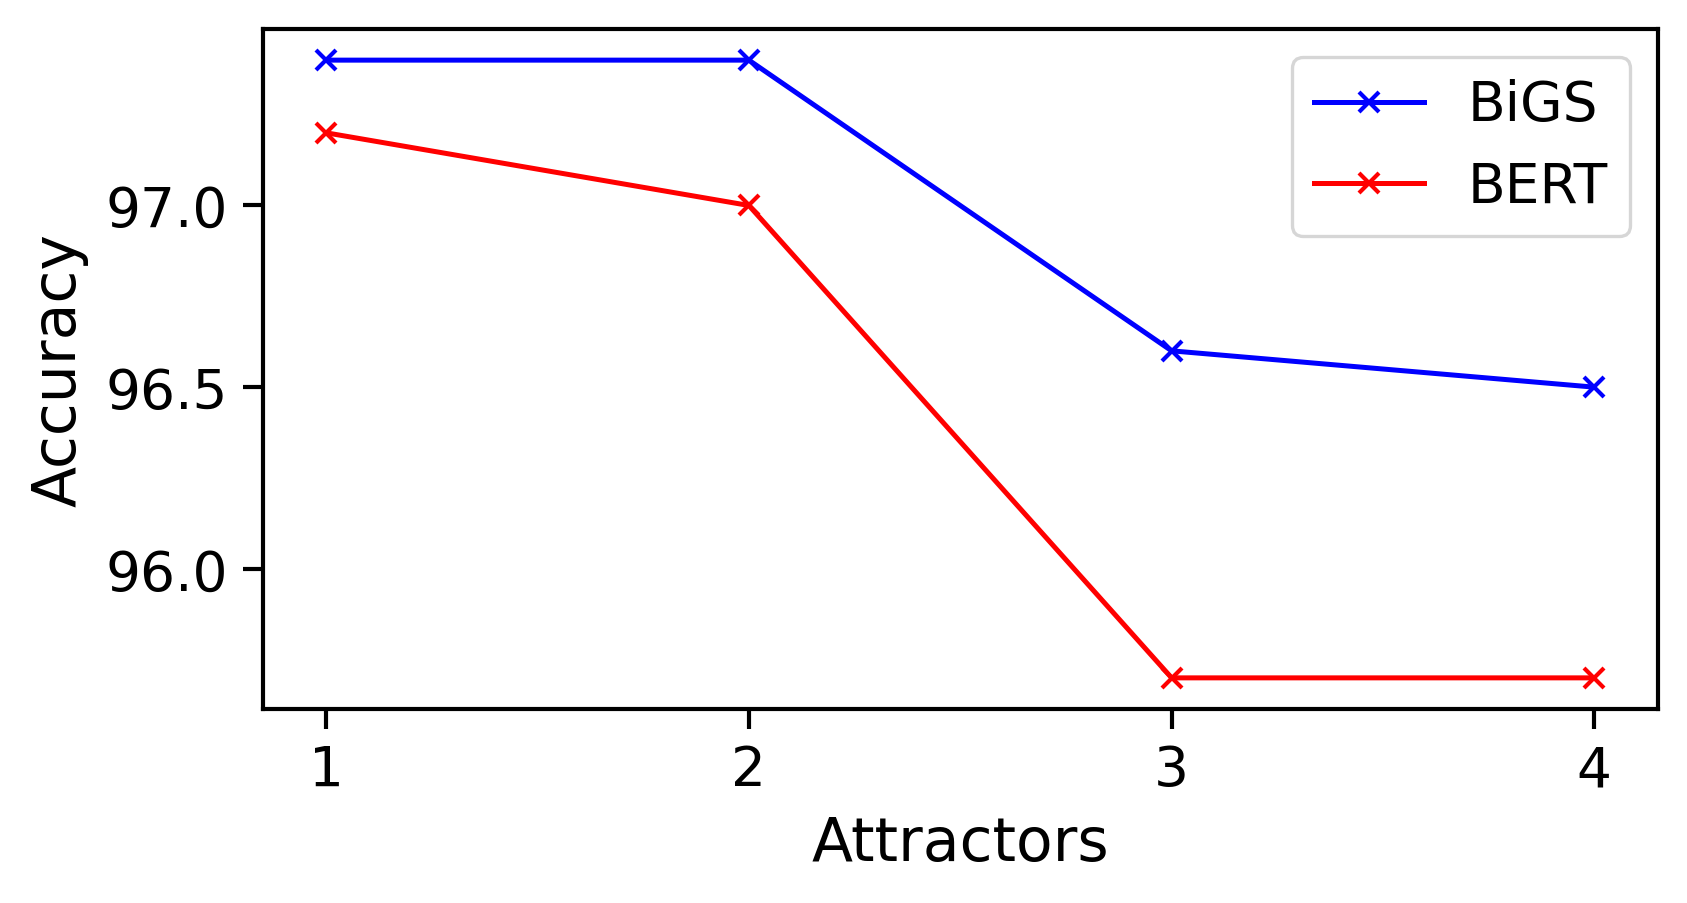
\includegraphics[height=0.5\textheight]{Figs/attractors.png}
        \label{fig:my_label}
    \end{figure}
    
\end{frame}

\begin{frame}{\structure{Observation 3}: Diagnostics }
From \cite{marvin2018targeted,goldberg2019assessing}:
\begin{table}[t]
\centering
\scriptsize
\begin{tabular}{lrrr}
\toprule
& BiGS & BERT & LSTM  \\
\midrule
\textsl{SUBJECT-VERB:}    &       &      &        \\
Simple                              & 100.0 & 100.0& 94.0    \\
Sentential complement          & 85.1  & 85.6 & 99.0   \\
Short VP coordination               & 91.0  & 86.5 & 90.0    \\
Long VP coordination                & 97.5  & 97.5 & 61.0    \\ 
Across prep phrase       & 88.6  & 84.8 & 57.0  \\ 
Across subj relative clause    & 88.4  & 84.9 & 56.0   \\
Across obj relative clause    & 89.9  & 85.1 & 50.0  \\
Across obj relative (-that) & 86.9  & 81.1 & 52.0  \\ 
In  obj relative clause        & 97.2  & 99.1 & 84.0  \\
In obj relative (-that)     & 88.7  & 81.6 & 71.0  \\
\midrule
\textsl{REFL ANAPHORA:}        &       &      &             \\
Simple                              & 97.1  & 98.9 & 83.0    \\
In a sentential complement          & 79.9  & 86.2 & 86.0   \\
Across a relative clause            & 79.1  & 75.9 & 55.0  \\
\bottomrule
\end{tabular}
\end{table}
\end{frame}


\begin{frame}{\structure{Experiment 2:} Longformer}
\begin{itemize}
    \item Can we lengthen SSM $L\rightarrow L'$ without approximation?
    
    \item Continued training based on Longformer protocol. 
    
    \item Two experimental scales
    % \begin{itemize}
    %     \item 128->512 SQuAD \cite{rajpurkar2016squad}
    %     \item 128->4096 SCROLLS \cite{shaham2022scrolls}
    % \end{itemize}
\end{itemize}
\end{frame}

% \begin{frame}{SQuAD}
% \begin{table}[tb]
%     \centering
%     \begin{tabular}{ll|c}
%     \toprule
%            & & SQuAD 1.1 \\
%     \midrule
%          BERT & (512) & 90.9\\
%          \midrule
%          BERT &(128 $\rightarrow$ 512) & 87.3 \\
%          BiGS &  (128 $\rightarrow$ 512) & 89.5 \\
%     \bottomrule
%     \end{tabular}
%     \caption{ }
%     \label{tab:squad}
% \end{table}    
% \end{frame}



\begin{frame}{SCROLLS}
    \begin{table}[tb]
    \centering
    \begin{tabular}{lr|cc}
    \toprule
        & Length & QALT & CNLI \\
    \midrule
         LED  & 1024    &  26.6/27.2  & 73.4\\
           & 4096    &  26.6/27.3  & 71.5\\
           & 16384   &  25.8/25.4   & 71.5\\
         \midrule
         BART & 256  &  26.0/25.8 & 69.8\\
          & 512  &  26.8/27.4 & 71.6\\
          & 1024 &  26.0/25.9 & 77.4\\
         \midrule
         BiGS & 128  & 32.3/30.0 & 68.7 \\
         % BiGS & 1024 &  & \\
          & 4096 & 32.8/31.7 & 71.4 \\
    \bottomrule
    \end{tabular}
    \caption{}
    \label{tab:scroll}
\end{table}
\end{frame}

\begin{frame}{FLOPs}
\begin{figure}
    \centering
    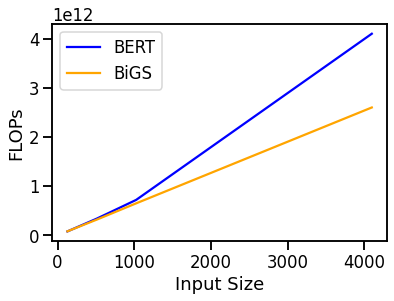
\includegraphics[height=0.5\textheight]{Figs/graph2.png}

    \label{fig:my_label}
\end{figure}
\end{frame}

\begin{frame}{Related Results: H3 - SSM For Language Modeling}
\begin{itemize}
    \item Alternative gating method for language modeling
    \item Use 2 attention layers + SSM and reach Transformer PPL. 
    \item Efficient implementation targeting on GPUs. 
\end{itemize}

    \blfootnote{\cite{dao2022hungry}}
\end{frame}


% \section{Next Steps}
% \begin{frame}{Outline}
%     \tableofcontents[currentsection]
% \end{frame}


\begin{frame}{Next Steps}
\begin{itemize}
    \item Attention may not be required? Simpler routing + gating. 
    \item More analysis on feed-forward contribution. 
    \item Transfer from pretraining unclear.
\end{itemize}
\end{frame}

% \begin{frame}
%     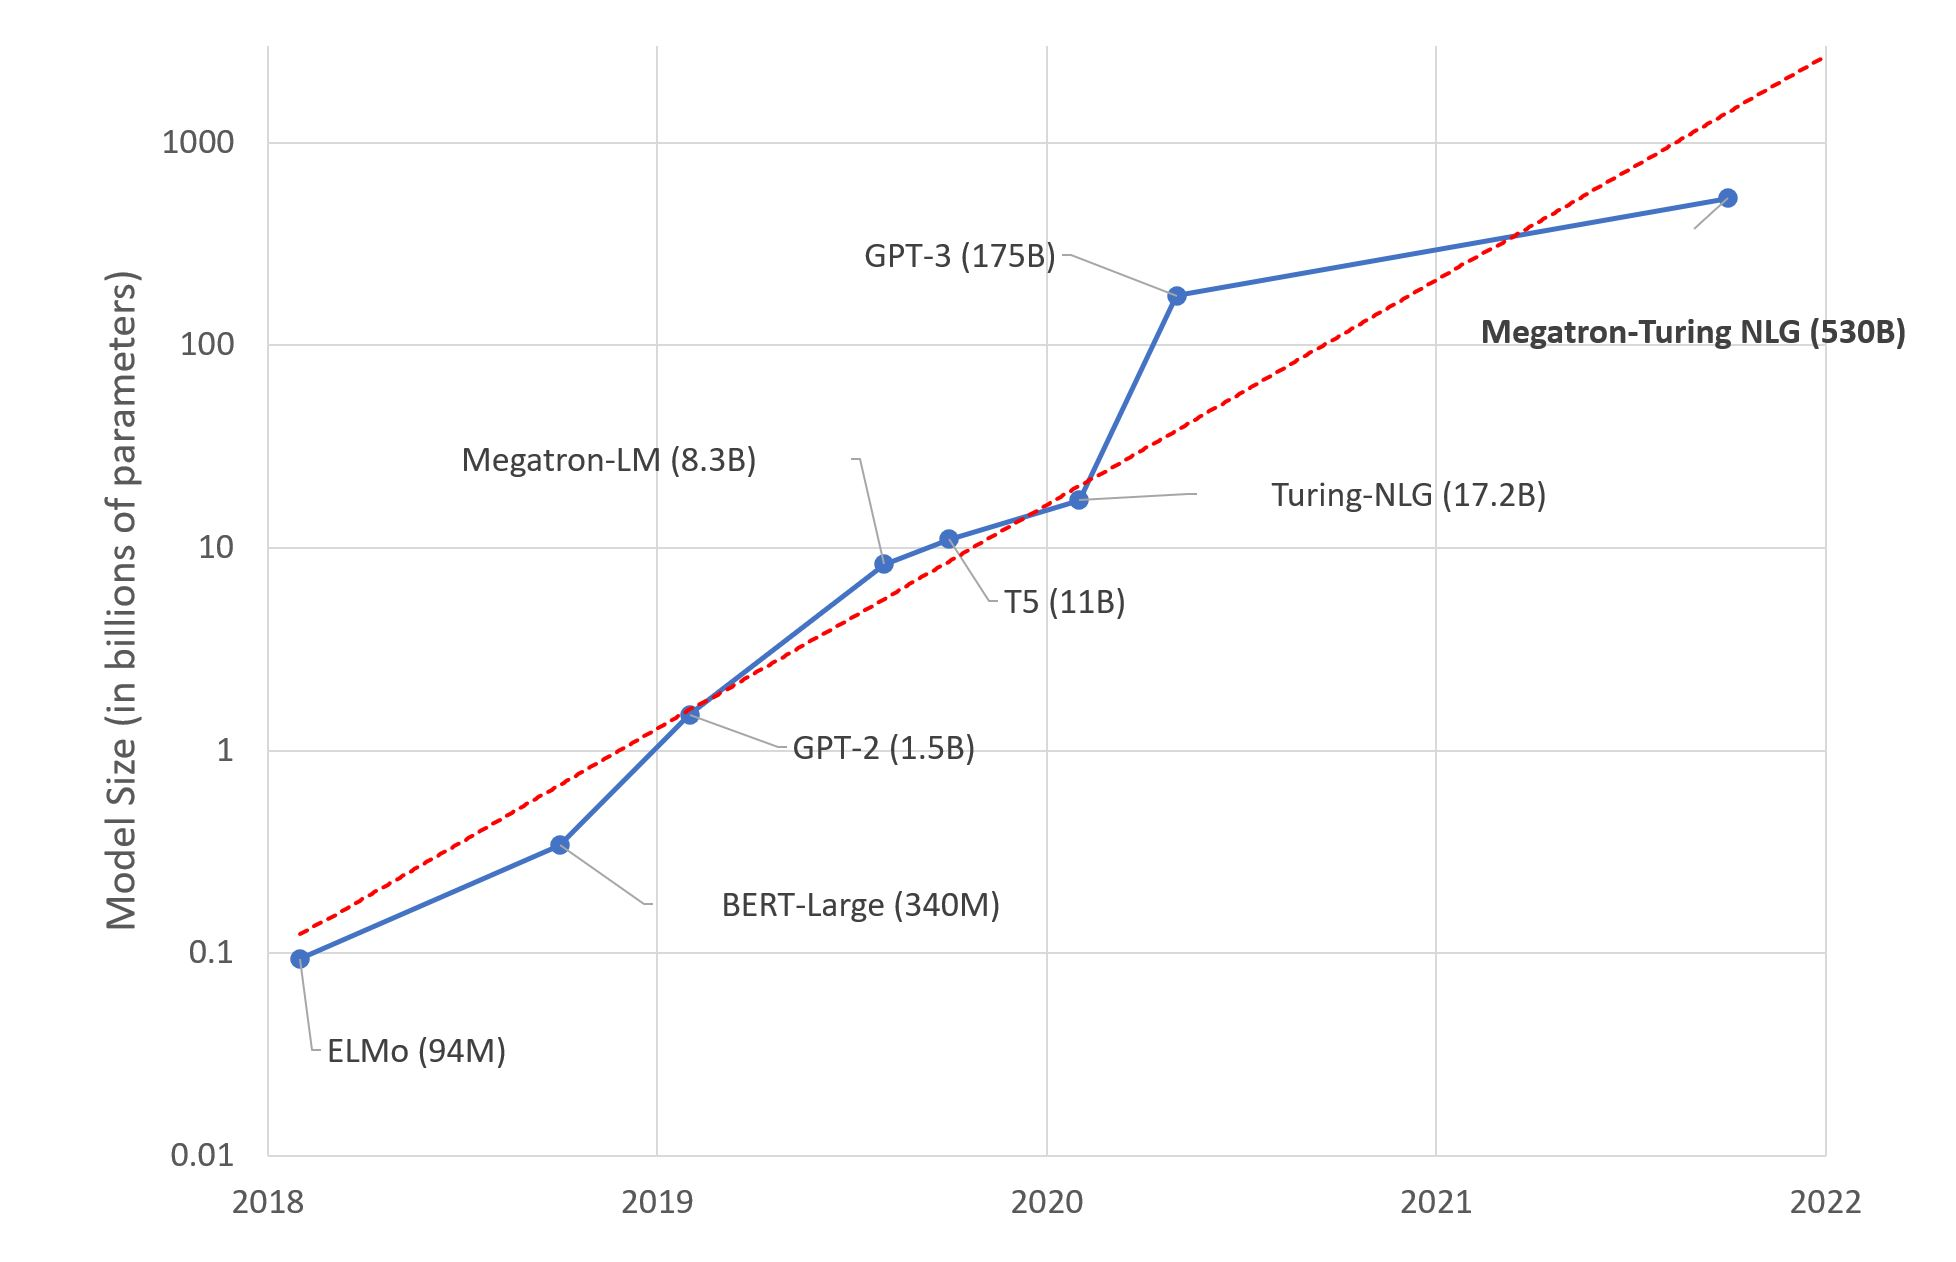
\includegraphics[height=\textheight]{Figs/ModelSize0.jpg}
% \end{frame}


% \begin{frame}{A slide title}

  \begin{itemize}
    \item A bulleted item
    \item Another item
      \begin{itemize}
        \item With sub-bullets
        \item And another, with some \textbf{bold} text
      \end{itemize}
    \item And another, at the top level, with \textit{italic} text
  \end{itemize}

  \note{
    Here's a note for this slide.
  }

\end{frame}

% \begin{frame}{A 50-50 split slide}

  \begin{columns}
    \begin{column}{0.5\linewidth}
      \begin{itemize}
        \item This side has a bullet
        \item And another bullet, with text that wraps if it's long
      \end{itemize}
    \end{column}
    \begin{column}{0.5\linewidth}
      \begin{figure}
        \centering
        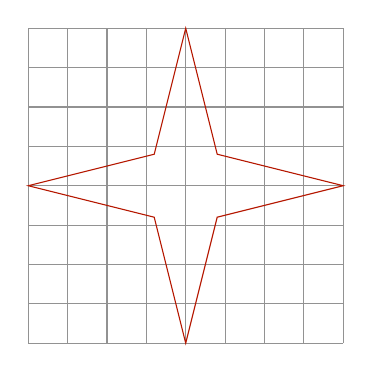
\begin{tikzpicture}[scale=2]
          \draw[step=0.25cm,color=gray] (-1,-1) grid (1,1);
          \draw[color=red] (1,0) -- (0.2,0.2) -- (0,1) -- (-0.2,0.2) -- (-1,0)
          -- (-0.2,-0.2) -- (0,-1) -- (0.2,-0.2) -- cycle;
        \end{tikzpicture}
        \caption{A figure caption}
      \end{figure}
    \end{column}
  \end{columns}

  \note{
    This slide has notes too.
  }

\end{frame}

% \begin{frame}{Full-slide figure}

  \begin{figure}
    \centering
    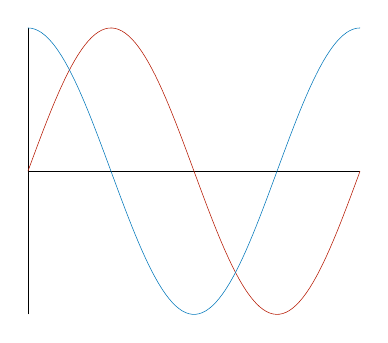
\begin{tikzpicture}[scale=0.5]
      \begin{axis}[
          scale only axis,
          no markers,
          domain=0:2*pi,
          samples=100,
          axis lines=center,
          axis line style={-},
          ticks=none]
        \addplot[red] {sin(deg(x))};
        \addplot[blue] {cos(deg(x))};
      \end{axis}
    \end{tikzpicture}
  \end{figure}
    \blfootnote{[Here is a citation]}


\end{frame}

% \begin{frame}{A slide with centered text}

  \begin{center}
    Some statement that is centered.
  \end{center}

  \vspace{2ex}
  \begin{center}
    \scriptsize (a small note)
  \end{center}

\end{frame}

% \begin{frame}[fragile]{A slide with some code}

	\begin{columns}
		\begin{column}{0.5\linewidth}
			\footnotesize
			\begin{Verbatim}[commandchars=\\\{\}]
/* some code */
def foo(x):
  return x**0.5 + 2*x

\color{blue}/* some can be highlighted */
\color{blue}foo(3)
      \end{Verbatim}
    \end{column}
    \begin{column}{0.5\linewidth}
      {\color{red} Some explanatory text, in red, with some \texttt{monospace} text.}
      There might be some math, too:

      $$\sqrt{x} + 2x$$
    \end{column}
  \end{columns}

\end{frame}

% \begin{frame}{A slide with some bracketed text}

	\begin{itemize}
		\item Some statement {\color{gray} [Some citation]}
		\item Another statement {\color{gray} [Another citation]}
		\item A final statement {\color{gray} [The last citation]}
	\end{itemize}

	\vspace{3ex}
	\begin{center}
		\scriptsize (a small note)
	\end{center}

\end{frame}


% \begin{frame}{A slide with some text and a link}

  \begin{itemize}
    \item This slide has some text along with a link
      \begin{itemize}
        \item \textbf{Some bold text}: followed by an explanation
        \item \textbf{More bold text}: followed by more text
      \end{itemize}
    \item Another bullet, with sub-bullets
      \begin{itemize}
        \item A sub-bullet
        \item Another sub-bullet, with more text
      \end{itemize}
  \end{itemize}

  \vspace{2ex}
  \begin{center}
    \color{blue} \href{https://github.com/anishathalye/auriga}{github.com/anishathalye/auriga}
  \end{center}

\end{frame}

\begin{frame}[allowframebreaks]
        \frametitle{References}
        \footnotesize
        \bibliographystyle{apalike}
        \bibliography{anthology.bib}
\end{frame}
\end{document}
